\documentclass[11pt, a4paper]{article}

% ===== Packages =====
\usepackage[utf8]{inputenc}
\usepackage[T1]{fontenc}
\usepackage{lmodern}
\usepackage[margin=0.75in]{geometry}
\usepackage{graphicx}
\usepackage{xcolor}
\usepackage{pagecolor}
\usepackage{hyperref}
\usepackage{listings}
\usepackage{tikz}
\usepackage{tcolorbox}
\usepackage{booktabs}
\usepackage{longtable}
\usepackage{fancyhdr}
\usepackage{enumitem}
\usepackage{amsmath}
\usepackage{float}

\usetikzlibrary{shapes.geometric, arrows.meta, positioning, fit, backgrounds, calc}

% ===== Colors =====
\definecolor{covenantblue}{HTML}{60A5FA}
\definecolor{covenantdark}{HTML}{F8FAFC}
\definecolor{covenantgray}{HTML}{94A3B8}
\definecolor{codebg}{HTML}{1E293B}
\definecolor{codeframe}{HTML}{334155}
\definecolor{keywordcolor}{HTML}{A78BFA}
\definecolor{stringcolor}{HTML}{34D399}
\definecolor{commentcolor}{HTML}{94A3B8}
\definecolor{successgreen}{HTML}{4ADE80}
\definecolor{warningyellow}{HTML}{FACC15}
\definecolor{dangerred}{HTML}{F87171}
\definecolor{infoblue}{HTML}{38BDF8}
\definecolor{pagebg}{HTML}{1E1E1E}
\definecolor{textmain}{HTML}{E0E0E0}

% ===== Hyperlinks =====
\hypersetup{
    colorlinks=true,
    linkcolor=covenantblue,
    urlcolor=covenantblue,
    citecolor=covenantblue,
    pdftitle={Covenant Platform -- Technical Guide},
    pdfauthor={Covenant Team}
}

% ===== Code Listings =====
\lstdefinestyle{javastyle}{
    language=Java,
    backgroundcolor=\color{codebg},
    frame=single,
    rulecolor=\color{codeframe},
    basicstyle=\ttfamily\footnotesize,
    keywordstyle=\color{keywordcolor}\bfseries,
    stringstyle=\color{stringcolor},
    commentstyle=\color{commentcolor}\itshape,
    breaklines=true,
    showstringspaces=false,
    tabsize=4,
    xleftmargin=1em,
    framexleftmargin=0.5em,
    numbers=left,
    numberstyle=\tiny\color{covenantgray},
    numbersep=8pt,
    aboveskip=1em,
    belowskip=1em,
    morekeywords={String, List, Optional, void, boolean, var, record}
}

\lstdefinestyle{yamlstyle}{
    basicstyle=\ttfamily\footnotesize,
    backgroundcolor=\color{codebg},
    frame=single,
    rulecolor=\color{codeframe},
    breaklines=true,
    showstringspaces=false,
    xleftmargin=1em,
    framexleftmargin=0.5em,
    aboveskip=1em,
    belowskip=1em,
    keywordstyle=\color{keywordcolor}\bfseries,
    commentstyle=\color{commentcolor}\itshape,
}

\lstset{style=javastyle}

% ===== Custom Boxes =====
\newtcolorbox{conceptbox}[1]{
    colback=infoblue!15!pagebg,
    coltext=textmain,
    colframe=infoblue,
    fonttitle=\bfseries,
    title=#1,
    arc=3pt,
    boxrule=1pt
}

\newtcolorbox{examplebox}[1]{
    colback=successgreen!15!pagebg,
    coltext=textmain,
    colframe=successgreen,
    fonttitle=\bfseries,
    title=Example: #1,
    arc=3pt,
    boxrule=1pt
}

\newtcolorbox{warningbox}[1]{
    colback=warningyellow!15!pagebg,
    coltext=textmain,
    colframe=warningyellow,
    fonttitle=\bfseries,
    title=Important: #1,
    arc=3pt,
    boxrule=1pt
}

\newtcolorbox{interviewbox}[1]{
    colback=keywordcolor!15!pagebg,
    coltext=textmain,
    colframe=keywordcolor,
    fonttitle=\bfseries,
    title=Interview Tip: #1,
    arc=3pt,
    boxrule=1pt
}

% ===== Headers & Footers =====
\pagestyle{fancy}
\fancyhf{}
\fancyhead[L]{\footnotesize\textcolor{covenantgray}{Covenant Platform -- Technical Guide}}
\fancyhead[R]{\footnotesize\textcolor{covenantgray}{\leftmark}}
\fancyfoot[C]{\thepage}

% ===== Tikz Styles =====
\tikzstyle{process} = [rectangle, rounded corners, minimum width=3cm, minimum height=1cm, text centered, draw=covenantblue, fill=covenantblue!25!pagebg, text=textmain, font=\small]
\tikzstyle{decision} = [diamond, minimum width=2.5cm, minimum height=1cm, text centered, draw=warningyellow, fill=warningyellow!25!pagebg, text=textmain, font=\small, aspect=2]
\tikzstyle{startstop} = [rectangle, rounded corners, minimum width=2.5cm, minimum height=0.8cm, text centered, draw=dangerred, fill=dangerred!25!pagebg, text=textmain, font=\small\bfseries]
\tikzstyle{io} = [trapezium, trapezium left angle=70, trapezium right angle=110, minimum width=2.5cm, minimum height=0.8cm, text centered, draw=successgreen, fill=successgreen!25!pagebg, text=textmain, font=\small]
\tikzstyle{arrow} = [thick, ->, >=Stealth, color=textmain]

% ============================================================
\begin{document}
\pagecolor{pagebg}
\color{textmain}

% ===== Title Page =====
\begin{titlepage}
\centering
\vspace*{2cm}

{\Huge\bfseries\textcolor{covenantdark}{Covenant Platform}\par}
\vspace{0.5cm}
{\Large\textcolor{covenantblue}{Secure Escrow Payment API}\par}
\vspace{1cm}
{\large\textcolor{covenantgray}{Complete Technical Reference Guide}\par}

\vspace{2cm}

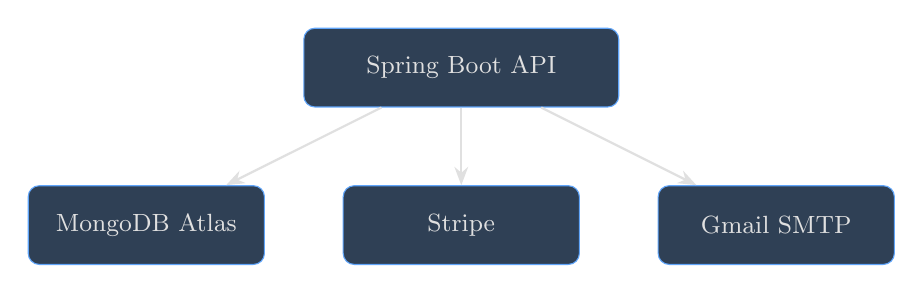
\begin{tikzpicture}
    % Architecture overview mini-diagram
    \node[process, minimum width=4cm] (api) at (0,0) {Spring Boot API};
    \node[process, minimum width=3cm] (db) at (-4,-2) {MongoDB Atlas};
    \node[process, minimum width=3cm] (stripe) at (0,-2) {Stripe};
    \node[process, minimum width=3cm] (email) at (4,-2) {Gmail SMTP};
    
    \draw[arrow] (api) -- (db);
    \draw[arrow] (api) -- (stripe);
    \draw[arrow] (api) -- (email);
\end{tikzpicture}

\vspace{2cm}

{\large Built With:\par}
\vspace{0.5cm}
\begin{tabular}{cccc}
    \textbf{Java 21} & \textbf{Spring Boot 3.5} & \textbf{MongoDB} & \textbf{Stripe API} \\
    \textbf{JWT Auth} & \textbf{Bucket4j} & \textbf{Lombok} & \textbf{Swagger/OpenAPI} \\
\end{tabular}

\vfill
{\small\textcolor{covenantgray}{Version 1.0 \quad|\quad \today}\par}
\end{titlepage}

\tableofcontents


% ============================================================
% CHAPTER 1: PROJECT OVERVIEW
% ============================================================
\section{Project Overview}

\subsection{What is Covenant Platform?}

Covenant is a \textbf{Secure Escrow Payment Platform} built as a REST API. In simple terms, it solves the \textit{trust problem} between online buyers and sellers.

\begin{conceptbox}{The Trust Problem}
Imagine you want to buy a laptop from a stranger on the internet.
\begin{itemize}
    \item If you pay first, the seller might never ship the laptop.
    \item If the seller ships first, you might never pay.
\end{itemize}
Neither party trusts the other. \textbf{Escrow} solves this by introducing a trusted third party (Covenant) that holds the money until both sides are happy.
\end{conceptbox}

\begin{examplebox}{How a Real Transaction Works}
\begin{enumerate}
    \item \textbf{Seller} creates a contract: ``Selling MacBook Pro for \rupee{}50,000''
    \item \textbf{Buyer} accepts the contract and pays \rupee{}50,000 via Stripe
    \item \textbf{Covenant} holds the money (status becomes \texttt{LOCKED})
    \item \textbf{Seller} ships the laptop and provides a tracking ID
    \item \textbf{Buyer} receives the laptop and clicks ``Satisfied''
    \item \textbf{Covenant} releases the \rupee{}50,000 to the Seller
\end{enumerate}
If the Buyer is unhappy, they can raise a \textbf{Dispute}, and an Admin resolves it.
\end{examplebox}

\newcommand{\rupee}{\textrm{\textup{INR~}}}

\subsection{Technology Stack}

\begin{longtable}{@{}lp{10cm}@{}}
\toprule
\textbf{Technology} & \textbf{Purpose} \\
\midrule
Java 21 & Core programming language (latest LTS version) \\
Spring Boot 3.5 & Web framework that auto-configures everything \\
MongoDB Atlas & Cloud-hosted NoSQL database for storing Users \& Contracts \\
Stripe API & Payment gateway for securely collecting money \\
JWT (jjwt 0.12.6) & Stateless authentication tokens \\
BCrypt & One-way password hashing algorithm \\
Bucket4j & Rate limiting library to prevent brute-force attacks \\
Lombok & Eliminates boilerplate code (getters, setters, constructors) \\
Spring Mail & Sending notification emails via Gmail SMTP \\
Swagger/OpenAPI & Auto-generated interactive API documentation \\
Maven & Build tool and dependency management \\
\bottomrule
\end{longtable}

\subsection{Project Structure}

The project follows the standard \textbf{Layered Architecture} pattern:

\begin{lstlisting}[style=yamlstyle, title={Directory Structure}]
com.covenant.platform/
|-- CovenantApplication.java        # Entry point
|-- config/                          # Configuration classes
|   |-- AppConfig.java               # Password encoder bean
|   |-- JwtAuthenticationFilter.java # JWT security filter
|   |-- SecurityConfig.java          # Spring Security setup
|-- controller/                      # REST API endpoints
|   |-- AuthController.java          # Login & Register
|   |-- ContractController.java      # All contract operations
|   |-- StripeWebhookController.java # Stripe payment callbacks
|-- dto/                             # Data Transfer Objects
|   |-- request/                     # Incoming request bodies
|   |-- response/                    # Outgoing response bodies
|-- entity/                          # MongoDB document models
|   |-- Contract.java                # Contract document
|   |-- TrackingDetails.java         # Embedded shipping info
|   |-- User.java                    # User document
|-- enums/                           # Status & Role enumerations
|-- exception/                       # Custom error handling
|-- repository/                      # MongoDB query interfaces
|-- scheduler/                       # Background cron jobs
|-- security/                        # Rate limiting filter
|-- service/                         # Core business logic
|-- util/                            # JWT utility methods
\end{lstlisting}

\begin{conceptbox}{Layered Architecture Explained}
Think of the application as a restaurant:
\begin{itemize}
    \item \textbf{Controller} = The Waiter (takes orders from customers, returns food)
    \item \textbf{Service} = The Chef (does the actual cooking/business logic)
    \item \textbf{Repository} = The Pantry (stores and retrieves ingredients/data)
    \item \textbf{Entity} = The Recipe Card (defines what a ``dish'' looks like)
    \item \textbf{DTO} = The Menu (what the customer sees -- not the raw ingredients)
\end{itemize}
The customer (API caller) never walks into the kitchen. They only talk to the waiter.
\end{conceptbox}


% ============================================================
% CHAPTER 2: DATABASE SCHEMA
% ============================================================
\section{Database Schema (MongoDB)}

MongoDB is a \textbf{NoSQL} document database. Instead of tables with rows and columns (like MySQL), it stores data as \textbf{JSON-like documents} inside \textbf{collections}.

\subsection{User Collection}

\begin{figure}[H]
\centering
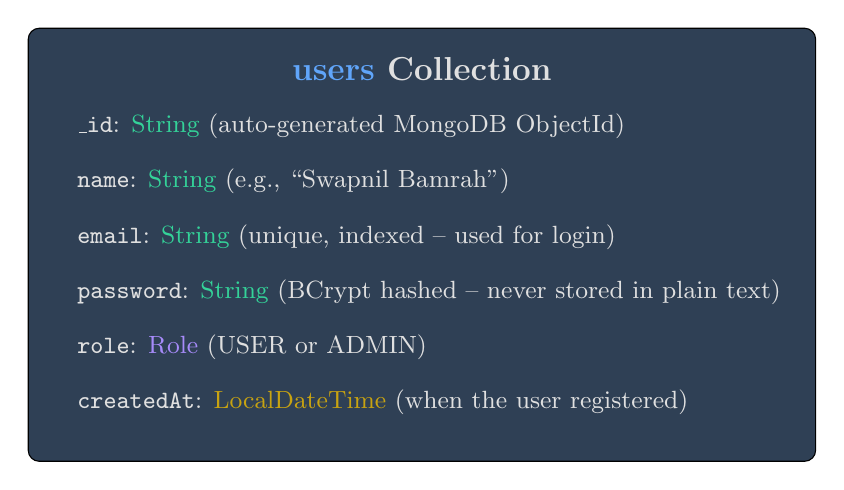
\begin{tikzpicture}[every node/.style={text=textmain, font=\small}]
    \node[draw, rounded corners, fill=covenantblue!25!pagebg, minimum width=10cm, minimum height=5.5cm] (box) at (0,0) {};
    \node[font=\bfseries\large, anchor=north] at (0,2.5) {\textcolor{covenantblue}{users} Collection};
    
    \node[anchor=west] at (-4.5,1.5) {\texttt{\_id}: \textcolor{stringcolor}{String} \textrm{(auto-generated MongoDB ObjectId)}};
    \node[anchor=west] at (-4.5,0.8) {\texttt{name}: \textcolor{stringcolor}{String} \textrm{(e.g., ``Swapnil Bamrah'')}};
    \node[anchor=west] at (-4.5,0.1) {\texttt{email}: \textcolor{stringcolor}{String} \textrm{(unique, indexed -- used for login)}};
    \node[anchor=west] at (-4.5,-0.6) {\texttt{password}: \textcolor{stringcolor}{String} \textrm{(BCrypt hashed -- never stored in plain text)}};
    \node[anchor=west] at (-4.5,-1.3) {\texttt{role}: \textcolor{keywordcolor}{Role} \textrm{(USER or ADMIN)}};
    \node[anchor=west] at (-4.5,-2.0) {\texttt{createdAt}: \textcolor{warningyellow!80!black}{LocalDateTime} \textrm{(when the user registered)}};
\end{tikzpicture}
\caption{User Document Structure}
\end{figure}

\begin{lstlisting}[caption={User.java -- The MongoDB Document Model}]
@Data                                 // Lombok: generates getters, setters, toString
@Document(collection = "users")       // Maps this class to the "users" collection
public class User {
    @Id
    private String id;                // MongoDB's auto-generated unique ID

    private String name;

    @Indexed(unique = true)           // Creates a unique index on email
    private String email;             // Used as the "username" for login

    private String password;          // BCrypt hashed (never plain text)

    private Role role = Role.USER;    // Default role for new users

    private LocalDateTime createdAt = LocalDateTime.now();
}
\end{lstlisting}

\begin{interviewbox}{Why is email indexed with \texttt{unique = true}?}
Two reasons:
\begin{enumerate}
    \item \textbf{Uniqueness}: Prevents two users from registering with the same email.
    \item \textbf{Performance}: MongoDB creates a B-Tree index on the email field, making \texttt{findByEmail()} queries extremely fast -- O(log n) instead of O(n).
\end{enumerate}
\end{interviewbox}

\subsection{Contract Collection}

\begin{figure}[H]
\centering
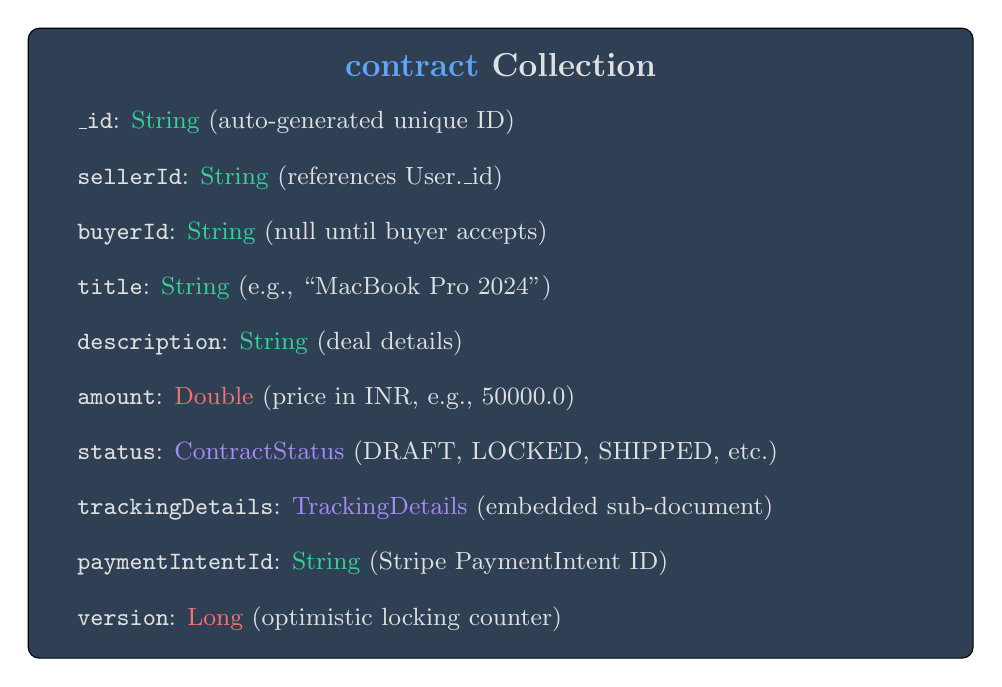
\begin{tikzpicture}[every node/.style={text=textmain, font=\small}]
    \node[draw, rounded corners, fill=covenantblue!25!pagebg, minimum width=12cm, minimum height=8cm] (box) at (0,0) {};
    \node[font=\bfseries\large, anchor=north] at (0,3.8) {\textcolor{covenantblue}{contract} Collection};
    
    \node[anchor=west] at (-5.5,2.8) {\texttt{\_id}: \textcolor{stringcolor}{String} \textrm{(auto-generated unique ID)}};
    \node[anchor=west] at (-5.5,2.1) {\texttt{sellerId}: \textcolor{stringcolor}{String} \textrm{(references User.\_id)}};
    \node[anchor=west] at (-5.5,1.4) {\texttt{buyerId}: \textcolor{stringcolor}{String} \textrm{(null until buyer accepts)}};
    \node[anchor=west] at (-5.5,0.7) {\texttt{title}: \textcolor{stringcolor}{String} \textrm{(e.g., ``MacBook Pro 2024'')}};
    \node[anchor=west] at (-5.5,0.0) {\texttt{description}: \textcolor{stringcolor}{String} \textrm{(deal details)}};
    \node[anchor=west] at (-5.5,-0.7) {\texttt{amount}: \textcolor{dangerred}{Double} \textrm{(price in INR, e.g., 50000.0)}};
    \node[anchor=west] at (-5.5,-1.4) {\texttt{status}: \textcolor{keywordcolor}{ContractStatus} \textrm{(DRAFT, LOCKED, SHIPPED, etc.)}};
    \node[anchor=west] at (-5.5,-2.1) {\texttt{trackingDetails}: \textcolor{keywordcolor}{TrackingDetails} \textrm{(embedded sub-document)}};
    \node[anchor=west] at (-5.5,-2.8) {\texttt{paymentIntentId}: \textcolor{stringcolor}{String} \textrm{(Stripe PaymentIntent ID)}};
    \node[anchor=west] at (-5.5,-3.5) {\texttt{version}: \textcolor{dangerred}{Long} \textrm{(optimistic locking counter)}};
\end{tikzpicture}
\caption{Contract Document Structure}
\end{figure}

\begin{conceptbox}{Embedded vs Referenced Documents}
Notice that \texttt{trackingDetails} is an \textbf{embedded} sub-document (stored inside the Contract document itself), while \texttt{sellerId}/\texttt{buyerId} are \textbf{references} (just storing the User's ID, not the entire User object).

\textbf{Rule of thumb}: Embed data that ``belongs'' to the parent and is always accessed together (like tracking info for a specific contract). Reference data that is shared across multiple documents (like a User who can have many contracts).
\end{conceptbox}

\subsubsection{TrackingDetails (Embedded Document)}

\begin{lstlisting}[caption={TrackingDetails.java}]
@Data @Builder @NoArgsConstructor @AllArgsConstructor
public class TrackingDetails {
    private String trackingId;          // e.g., "AWB123456789"
    private String logisticsProvider;   // e.g., "Delhivery"
    private LocalDateTime deliveryDate; // Set when seller marks as delivered
}
\end{lstlisting}

\subsection{Contract Status State Machine}

The \texttt{ContractStatus} enum defines a finite state machine with 9 possible states:

\begin{figure}[H]
\centering
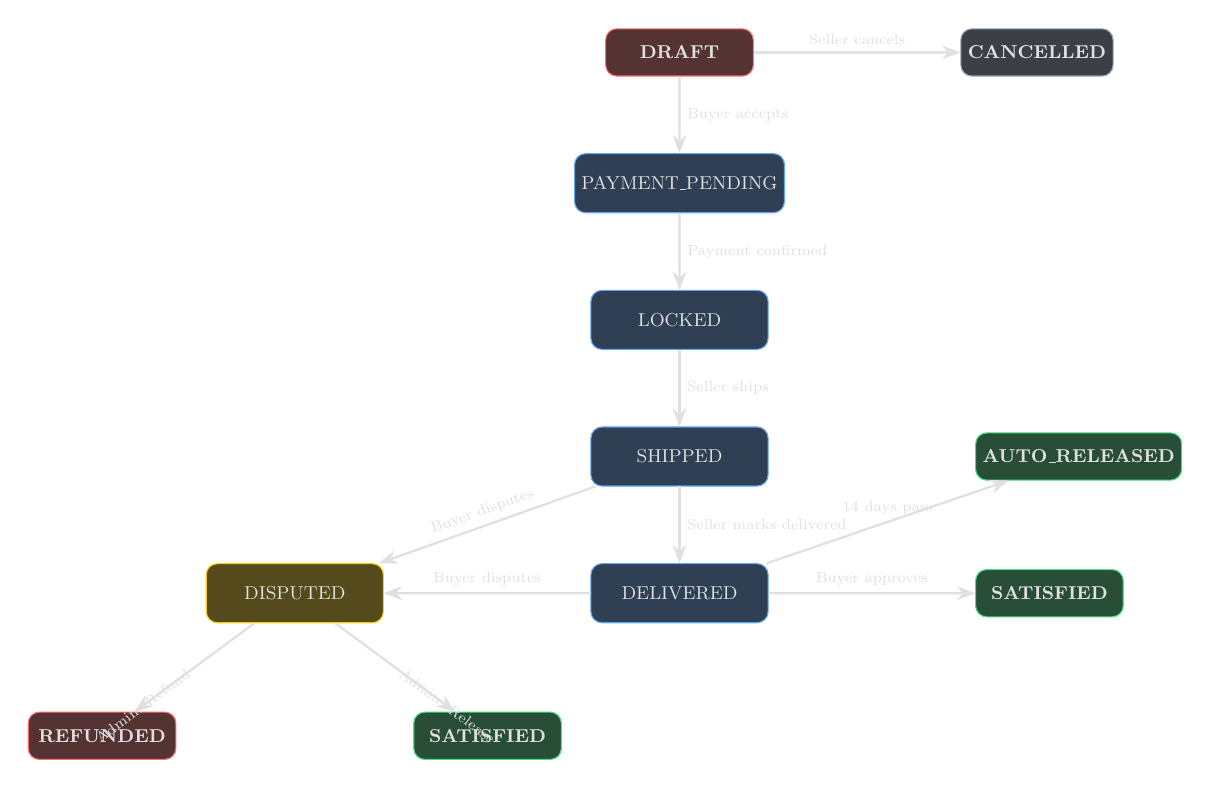
\begin{tikzpicture}[node distance=1.3cm, auto, every node/.style={text=textmain, font=\scriptsize}, scale=0.75, transform shape]
    % Nodes
    \node[startstop] (draft) {DRAFT};
    \node[process, below=of draft] (pending) {PAYMENT\_PENDING};
    \node[process, below=of pending] (locked) {LOCKED};
    \node[process, below=of locked] (shipped) {SHIPPED};
    \node[process, below=of shipped] (delivered) {DELIVERED};
    
    % Right side -- outcomes
    \node[startstop, right=3.5cm of delivered, fill=successgreen!25!pagebg, draw=successgreen] (satisfied) {SATISFIED};
    \node[startstop, right=3.5cm of shipped, fill=successgreen!25!pagebg, draw=successgreen] (autoreleased) {AUTO\_RELEASED};
    \node[process, left=3.5cm of delivered, fill=warningyellow!25!pagebg, draw=warningyellow] (disputed) {DISPUTED};
    
    % Bottom outcomes
    \node[startstop, below left=1.5cm and 0.5cm of disputed, fill=dangerred!25!pagebg, draw=dangerred] (refunded) {REFUNDED};
    \node[startstop, below right=1.5cm and 0.5cm of disputed, fill=successgreen!25!pagebg, draw=successgreen] (resolved) {SATISFIED};
    
    % Cancelled
    \node[startstop, right=3.5cm of draft, fill=covenantgray!25!pagebg, draw=covenantgray] (cancelled) {CANCELLED};
    
    % Arrows
    \draw[arrow] (draft) -- node[right] {Buyer accepts} (pending);
    \draw[arrow] (pending) -- node[right] {Payment confirmed} (locked);
    \draw[arrow] (locked) -- node[right] {Seller ships} (shipped);
    \draw[arrow] (shipped) -- node[right] {Seller marks delivered} (delivered);
    \draw[arrow] (delivered) -- node[above] {Buyer approves} (satisfied);
    \draw[arrow] (delivered) -- node[above] {14 days pass} (autoreleased);
    \draw[arrow] (delivered) -- node[above] {Buyer disputes} (disputed);
    \draw[arrow] (shipped) -- node[above, sloped] {Buyer disputes} (disputed);
    \draw[arrow] (disputed) -- node[left, sloped] {Admin: Refund} (refunded);
    \draw[arrow] (disputed) -- node[right, sloped] {Admin: Release} (resolved);
    \draw[arrow] (draft) -- node[above] {Seller cancels} (cancelled);
\end{tikzpicture}
\caption{Contract Lifecycle State Machine}
\end{figure}

\begin{lstlisting}[caption={ContractStatus.java}]
public enum ContractStatus {
    DRAFT,            // 1. Seller creates the contract
    PAYMENT_PENDING,  // 2. Buyer accepts, waiting for payment
    LOCKED,           // 3. Money received & held by Covenant

    SHIPPED,          // 4. Seller provided a Tracking ID
    DELIVERED,        // 5. Courier confirms delivery (Timer starts)

    SATISFIED,        // 6a. Buyer explicitly approves -> Release Money
    AUTO_RELEASED,    // 6b. 14 days passed with no dispute -> Release Money

    DISPUTED,         // 7. Buyer flagged an issue (Money frozen)
    CANCELLED,        // 8. Deal cancelled before payment
    REFUNDED          // 9. Money sent back to Buyer
}
\end{lstlisting}


% ============================================================
% CHAPTER 3: AUTHENTICATION & SECURITY
% ============================================================
\section{Authentication \& Security}

This chapter explains how the application verifies user identity and protects endpoints.

\subsection{Overview: What Happens When You Log In?}

\begin{figure}[H]
\centering
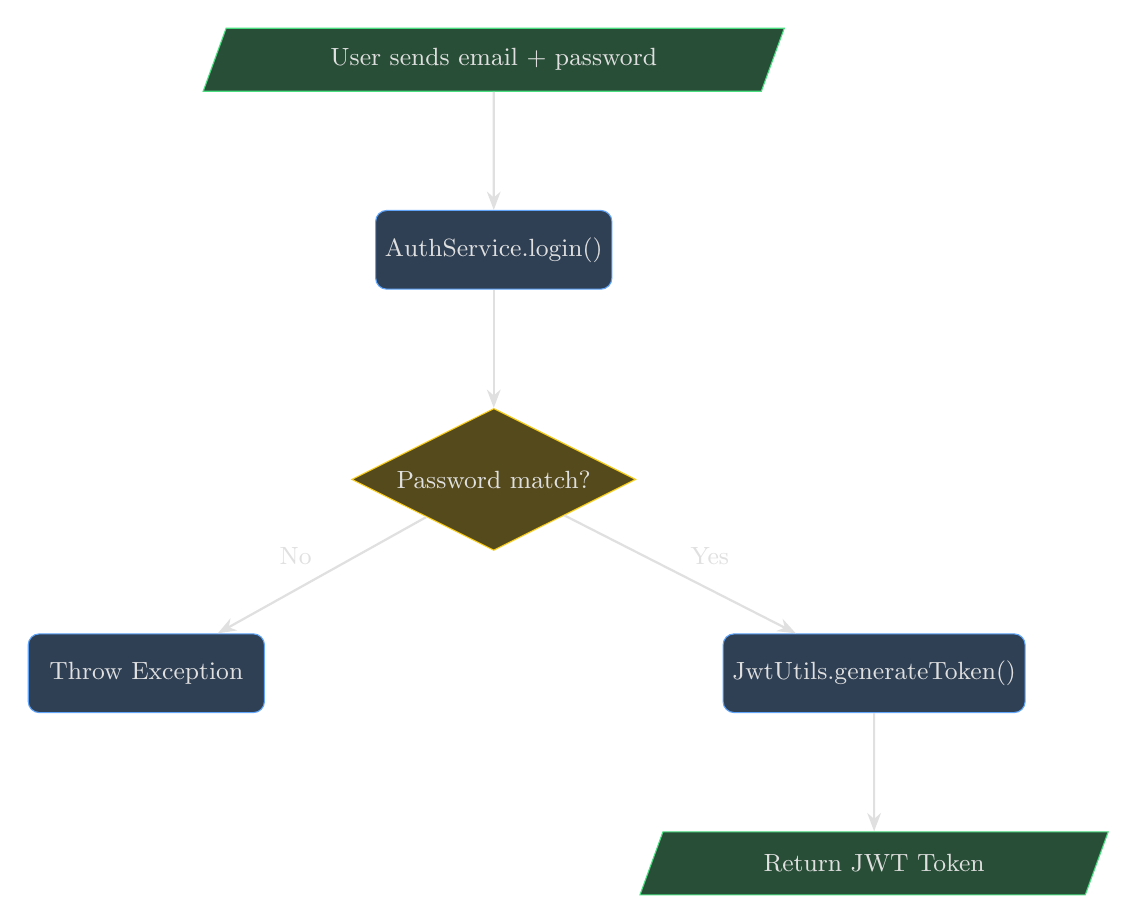
\begin{tikzpicture}[node distance=1.5cm, every node/.style={text=textmain, font=\small}]
    \node[io] (req) {User sends email + password};
    \node[process, below=of req] (auth) {AuthService.login()};
    \node[decision, below=of auth] (check) {Password match?};
    \node[process, below left=1.5cm and 2cm of check] (fail) {Throw Exception};
    \node[process, below right=1.5cm and 2cm of check] (jwt) {JwtUtils.generateToken()};
    \node[io, below=of jwt] (resp) {Return JWT Token};
    
    \draw[arrow] (req) -- (auth);
    \draw[arrow] (auth) -- (check);
    \draw[arrow] (check) -- node[above left] {No} (fail);
    \draw[arrow] (check) -- node[above right] {Yes} (jwt);
    \draw[arrow] (jwt) -- (resp);
\end{tikzpicture}
\caption{Login Flow}
\end{figure}

\subsection{Password Hashing with BCrypt}

Passwords are \textbf{never stored in plain text}. When a user registers, their password is hashed using BCrypt before being saved to MongoDB.

\begin{lstlisting}[caption={AppConfig.java -- BCrypt Bean}]
@Configuration
public class AppConfig {
    @Bean
    PasswordEncoder passwordEncoder() {
        return new BCryptPasswordEncoder();
    }
}
\end{lstlisting}

\begin{examplebox}{BCrypt in Action}
User registers with password: \texttt{MyPassword123}

Stored in MongoDB as: \texttt{\$2a\$10\$N9qo8uLOickgx2ZMRZoMye...}

Even if a hacker steals the entire database, they cannot reverse the hash back to the original password. BCrypt is a \textbf{one-way function}.
\end{examplebox}

\begin{lstlisting}[caption={AuthService.java -- Registration (Hashing the Password)}]
public UserResponse register(RegisterRequest request) {
    // 1. Check if email already exists
    if (userRepository.existsByEmail(request.getEmail())) {
        throw new IllegalStateException("Email already in use");
    }

    // 2. Create User entity
    User user = new User();
    user.setName(request.getName());
    user.setEmail(request.getEmail());
    user.setRole(Role.USER);

    // 3. Hash the password before saving (NEVER store plain text)
    user.setPassword(passwordEncoder.encode(request.getPassword()));

    // 4. Save to MongoDB
    User savedUser = userRepository.save(user);
    // 5. Return response (WITHOUT the password)
    return UserResponse.builder()
            .id(savedUser.getId())
            .name(savedUser.getName())
            .email(savedUser.getEmail())
            .role(savedUser.getRole())
            .createdAt(savedUser.getCreatedAt())
            .build();
}
\end{lstlisting}

\begin{interviewbox}{Why BCrypt and not SHA-256?}
SHA-256 is fast -- a GPU can compute billions of SHA-256 hashes per second. BCrypt is \textbf{intentionally slow} (it uses a ``cost factor'' to control speed). This makes brute-force attacks impractical. Even if an attacker knows the hash, trying every possible password would take years.
\end{interviewbox}

\subsection{JWT (JSON Web Tokens)}

After login, the server issues a \textbf{JWT} -- a compact, self-contained token that proves the user's identity for 24 hours.

\subsubsection{How JwtUtils.java Works}

\begin{lstlisting}[caption={JwtUtils.java -- Token Generation and Validation}]
@Component
public class JwtUtils {

    @Value("${jwt.secret}")
    private String secret;              // Base64-encoded secret from env

    private SecretKey key;              // HMAC-SHA key derived from secret

    private final long EXPIRATION_TIME = 86400000; // 24 hours in ms

    @PostConstruct
    public void init() {
        // Decode the Base64 secret and create an HMAC signing key
        byte[] keyBytes = Decoders.BASE64.decode(secret);
        this.key = Keys.hmacShaKeyFor(keyBytes);
    }

    // --- GENERATE TOKEN ---
    public String generateToken(String email) {
        return Jwts.builder()
                .subject(email)               // WHO this token belongs to
                .issuedAt(new Date())          // WHEN it was created
                .expiration(new Date(          // WHEN it expires (24h)
                    System.currentTimeMillis() + EXPIRATION_TIME))
                .signWith(key)                 // SIGN with our secret key
                .compact();                    // Build the final string
    }

    // --- VALIDATE TOKEN ---
    public boolean validateToken(String token, String userEmail) {
        final String username = extractUsername(token);
        return (username.equals(userEmail) && !isTokenExpired(token));
    }

    // --- EXTRACT USERNAME (email) FROM TOKEN ---
    public String extractUsername(String token) {
        return extractClaim(token, Claims::getSubject);
    }
}
\end{lstlisting}

\begin{conceptbox}{JWT Structure (3 Parts, separated by dots)}
A JWT looks like this: \texttt{xxxxx.yyyyy.zzzzz}

\begin{enumerate}
    \item \textbf{Header} (xxxxx): Algorithm used (HS256) and token type (JWT)
    \item \textbf{Payload} (yyyyy): The data -- user's email, issued time, expiry time
    \item \textbf{Signature} (zzzzz): HMAC-SHA256 of (Header + Payload + Secret Key)
\end{enumerate}

The signature ensures nobody can tamper with the payload. If someone changes the email inside the token, the signature won't match, and the server will reject it.
\end{conceptbox}

\subsection{The JWT Authentication Filter}

This is the ``Security Guard'' that checks every incoming HTTP request.

\begin{figure}[H]
\centering
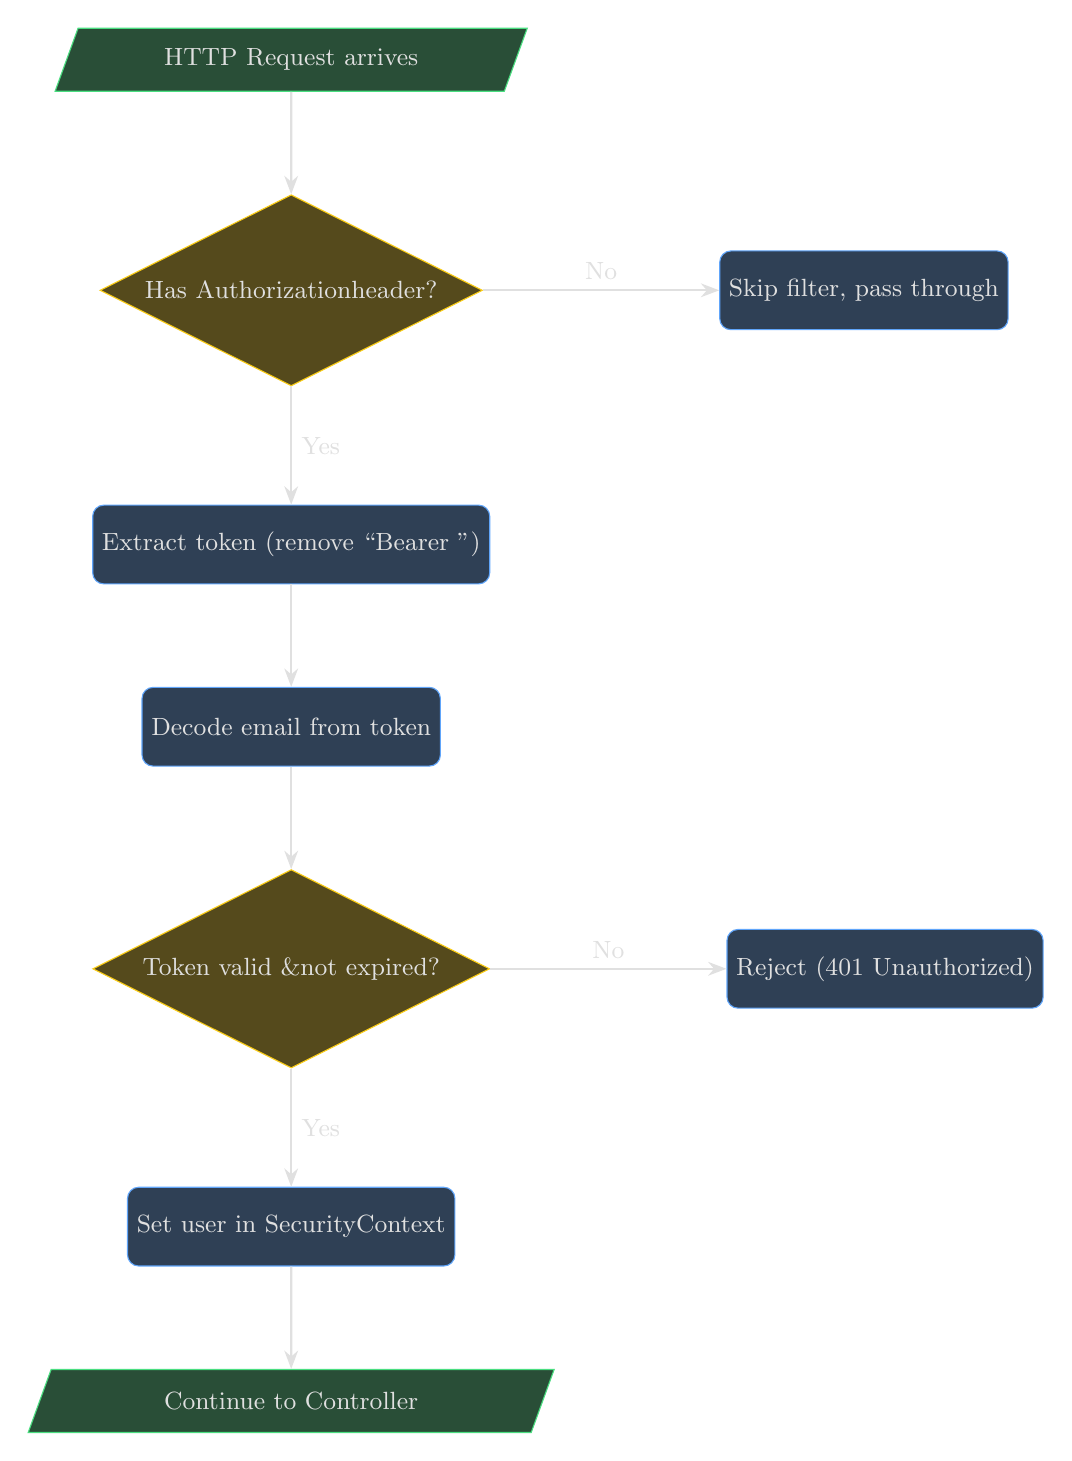
\begin{tikzpicture}[node distance=1.3cm, every node/.style={text=textmain, font=\small}]
    \node[io] (req) {HTTP Request arrives};
    \node[decision, below=of req] (header) {Has Authorization\\header?};
    \node[process, right=3cm of header] (skip) {Skip filter, pass through};
    \node[process, below=1.5cm of header] (extract) {Extract token (remove ``Bearer '')};
    \node[process, below=of extract] (decode) {Decode email from token};
    \node[decision, below=of decode] (valid) {Token valid \&\\not expired?};
    \node[process, right=3cm of valid] (reject) {Reject (401 Unauthorized)};
    \node[process, below=1.5cm of valid] (setauth) {Set user in SecurityContext};
    \node[io, below=of setauth] (continue) {Continue to Controller};
    
    \draw[arrow] (req) -- (header);
    \draw[arrow] (header) -- node[above] {No} (skip);
    \draw[arrow] (header) -- node[right] {Yes} (extract);
    \draw[arrow] (extract) -- (decode);
    \draw[arrow] (decode) -- (valid);
    \draw[arrow] (valid) -- node[above] {No} (reject);
    \draw[arrow] (valid) -- node[right] {Yes} (setauth);
    \draw[arrow] (setauth) -- (continue);
\end{tikzpicture}
\caption{JWT Authentication Filter Flow}
\end{figure}

\begin{lstlisting}[caption={JwtAuthenticationFilter.java -- The Security Guard}]
@Component
@RequiredArgsConstructor
public class JwtAuthenticationFilter extends OncePerRequestFilter {

    private final JwtUtils jwtUtils;
    private final CustomUserDetailsService userDetailsService;

    @Override
    protected void doFilterInternal(HttpServletRequest request,
                                    HttpServletResponse response,
                                    FilterChain filterChain)
            throws ServletException, IOException {

        // 1. Get the Authorization header
        final String authHeader = request.getHeader("Authorization");
        final String jwt;
        final String userEmail;

        // 2. If no header or doesn't start with "Bearer ", skip this filter
        if (authHeader == null || !authHeader.startsWith("Bearer ")) {
            filterChain.doFilter(request, response);
            return;
        }

        // 3. Extract the token (everything after "Bearer ")
        jwt = authHeader.substring(7);
        userEmail = jwtUtils.extractUsername(jwt);

        // 4. If email exists and user is NOT already authenticated
        if (userEmail != null &&
            SecurityContextHolder.getContext().getAuthentication() == null) {

            UserDetails userDetails =
                this.userDetailsService.loadUserByUsername(userEmail);

            // 5. Validate the token
            if (jwtUtils.validateToken(jwt, userDetails.getUsername())) {
                // 6. Create auth token and set in SecurityContext
                UsernamePasswordAuthenticationToken authToken =
                    new UsernamePasswordAuthenticationToken(
                        userDetails, null, userDetails.getAuthorities());

                authToken.setDetails(
                    new WebAuthenticationDetailsSource().buildDetails(request));

                // THE MAGIC MOMENT: User is now "logged in" for this request
                SecurityContextHolder.getContext().setAuthentication(authToken);
            }
        }

        filterChain.doFilter(request, response);
    }
}
\end{lstlisting}

\begin{interviewbox}{Why ``Stateless'' JWT instead of Sessions?}
With sessions, the server stores login state in memory. If you have 3 servers behind a load balancer, a user might log in on Server 1 but their next request goes to Server 2, which has no idea who they are.

With JWT, the token contains all the user info. Any server can validate it independently using the shared secret key. This is why JWT is \textbf{stateless} and ideal for scalable microservices.
\end{interviewbox}

\subsection{Spring Security Configuration}

\begin{lstlisting}[caption={SecurityConfig.java -- Defining Access Rules}]
@Configuration
@EnableWebSecurity
@RequiredArgsConstructor
public class SecurityConfig {

    private final JwtAuthenticationFilter jwtAuthFilter;
    private final RateLimitingFilter rateLimitingFilter;

    @Bean
    public SecurityFilterChain securityFilterChain(HttpSecurity http)
            throws Exception {
        http
            .csrf(AbstractHttpConfigurer::disable)  // Disable CSRF for REST APIs
            .authorizeHttpRequests(auth -> auth
                // Public endpoints (no login required)
                .requestMatchers("/api/auth/**").permitAll()
                .requestMatchers("/api/webhooks/stripe").permitAll()
                .requestMatchers("/v3/api-docs/**", "/swagger-ui/**",
                                 "/swagger-ui.html").permitAll()
                .requestMatchers("/actuator/**").permitAll()
                // Everything else requires authentication
                .anyRequest().authenticated()
            )
            .sessionManagement(session -> session
                // STATELESS = No cookies, no sessions. Pure JWT.
                .sessionCreationPolicy(SessionCreationPolicy.STATELESS)
            )
            // Add filters in order: Rate Limiting -> JWT -> Controller
            .addFilterBefore(rateLimitingFilter,
                UsernamePasswordAuthenticationFilter.class)
            .addFilterBefore(jwtAuthFilter,
                UsernamePasswordAuthenticationFilter.class);
        return http.build();
    }
}
\end{lstlisting}

\begin{warningbox}{Why is CSRF disabled?}
CSRF (Cross-Site Request Forgery) protection is designed for \textbf{browser-based} applications that use cookies. Since our API uses JWT tokens (sent in the \texttt{Authorization} header, not cookies), CSRF attacks are not possible. Disabling it is the standard practice for stateless REST APIs.
\end{warningbox}

\subsection{Rate Limiting with Bucket4j}

The Rate Limiting Filter prevents brute-force attacks by limiting how many requests a single IP address can make per minute.

\begin{lstlisting}[caption={RateLimitingFilter.java -- Token Bucket Algorithm}]
@Component
@Slf4j
public class RateLimitingFilter extends OncePerRequestFilter {

    // Separate buckets for register and login endpoints
    private final Map<String, Bucket> registerBuckets = new ConcurrentHashMap<>();
    private final Map<String, Bucket> loginBuckets = new ConcurrentHashMap<>();

    @Override
    protected void doFilterInternal(HttpServletRequest request,
            HttpServletResponse response,
            FilterChain filterChain) throws ServletException, IOException {

        String path = request.getRequestURI();
        String clientIp = getClientIp(request);

        Bucket bucket = null;

        if ("/api/auth/register".equals(path)) {
            // Allow 5 registration attempts per minute per IP
            bucket = registerBuckets.computeIfAbsent(clientIp,
                k -> createBucket(5));
        } else if ("/api/auth/login".equals(path)) {
            // Allow 10 login attempts per minute per IP
            bucket = loginBuckets.computeIfAbsent(clientIp,
                k -> createBucket(10));
        }

        if (bucket != null) {
            ConsumptionProbe probe = bucket.tryConsumeAndReturnRemaining(1);
            if (!probe.isConsumed()) {
                // Rate limit exceeded! Return 429 Too Many Requests
                response.setStatus(HttpStatus.TOO_MANY_REQUESTS.value());
                // ... write error JSON response ...
                return;   // STOP! Don't forward to the controller.
            }
        }

        filterChain.doFilter(request, response);  // All good, proceed.
    }

    private Bucket createBucket(int capacityPerMinute) {
        Bandwidth limit = Bandwidth.builder()
                .capacity(capacityPerMinute)
                .refillGreedy(capacityPerMinute, Duration.ofMinutes(1))
                .build();
        return Bucket.builder().addLimit(limit).build();
    }
}
\end{lstlisting}

\begin{conceptbox}{The Token Bucket Algorithm}
Imagine a bucket that can hold 10 tokens. Every minute, the bucket is refilled to 10 tokens. Each API request ``consumes'' 1 token. If the bucket is empty (0 tokens), the request is rejected with HTTP 429 (Too Many Requests).

\begin{center}
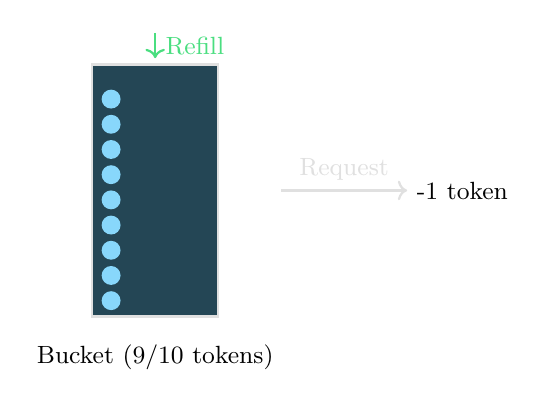
\begin{tikzpicture}[scale=0.8]
    \draw[thick, textmain, fill=infoblue!25!pagebg] (0,0) rectangle (2,4);
    \foreach \y in {0.4,0.8,1.2,1.6,2.0,2.4,2.8,3.2,3.6}
        \fill[infoblue!60] (0.3,\y-0.15) circle (0.15);
    \node[below] at (1,-0.3) {\small Bucket (9/10 tokens)};
    \draw[->, thick, textmain] (3,2) -- (5,2) node[midway, above] {\small Request};
    \node[right] at (5,2) {\small -1 token};
    
    \draw[->, thick, successgreen] (1,4.5) -- (1,4.1) node[midway, right] {\small Refill};
\end{tikzpicture}
\end{center}

\textbf{Why \texttt{ConcurrentHashMap}}? Multiple users send requests simultaneously (concurrently). A regular \texttt{HashMap} is not thread-safe and could corrupt data. \texttt{ConcurrentHashMap} handles simultaneous reads/writes safely.
\end{conceptbox}

\begin{interviewbox}{Why only rate-limit /login and /register?}
These are the only \textbf{public} endpoints (no JWT required). An attacker could try millions of passwords on \texttt{/login} without any authentication. Contract endpoints already require a valid JWT, so a brute-force attack on them is much harder -- the attacker would first need to steal a token.
\end{interviewbox}

\subsection{The Complete Request Pipeline}

Every HTTP request passes through these layers in order:

\begin{figure}[H]
\centering
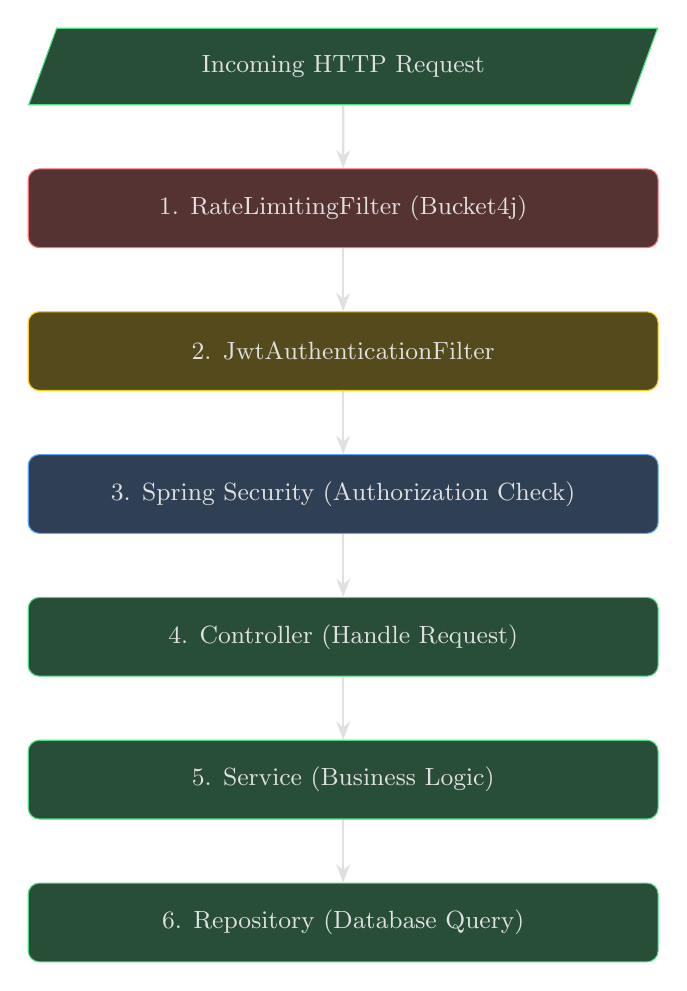
\begin{tikzpicture}[node distance=0.8cm, every node/.style={text=textmain, font=\small}]
    \node[io, minimum width=8cm] (req) {Incoming HTTP Request};
    \node[process, below=of req, minimum width=8cm, fill=dangerred!25!pagebg, draw=dangerred] (rate) {1. RateLimitingFilter (Bucket4j)};
    \node[process, below=of rate, minimum width=8cm, fill=warningyellow!25!pagebg, draw=warningyellow] (jwt) {2. JwtAuthenticationFilter};
    \node[process, below=of jwt, minimum width=8cm, fill=covenantblue!25!pagebg, draw=covenantblue] (security) {3. Spring Security (Authorization Check)};
    \node[process, below=of security, minimum width=8cm, fill=successgreen!25!pagebg, draw=successgreen] (controller) {4. Controller (Handle Request)};
    \node[process, below=of controller, minimum width=8cm, fill=successgreen!25!pagebg, draw=successgreen] (service) {5. Service (Business Logic)};
    \node[process, below=of service, minimum width=8cm, fill=successgreen!25!pagebg, draw=successgreen] (repo) {6. Repository (Database Query)};
    
    \draw[arrow] (req) -- (rate);
    \draw[arrow] (rate) -- (jwt);
    \draw[arrow] (jwt) -- (security);
    \draw[arrow] (security) -- (controller);
    \draw[arrow] (controller) -- (service);
    \draw[arrow] (service) -- (repo);
\end{tikzpicture}
\caption{Complete Request Pipeline}
\end{figure}


% ============================================================
% CHAPTER 4: CONTROLLERS (REST API Endpoints)
% ============================================================
\section{Controllers (REST API Endpoints)}

Controllers are the ``front door'' of the application. They receive HTTP requests, delegate work to the Service layer, and return HTTP responses.

\subsection{AuthController}

Handles user registration and login. Both endpoints are \textbf{public} (no JWT required).

\begin{longtable}{@{}llp{7cm}@{}}
\toprule
\textbf{Method} & \textbf{Endpoint} & \textbf{Description} \\
\midrule
POST & \texttt{/api/auth/register} & Register a new user. Accepts name, email, password. Returns user info (no password). \\
POST & \texttt{/api/auth/login} & Authenticate a user. Accepts email + password. Returns a JWT token. \\
\bottomrule
\end{longtable}

\begin{lstlisting}[caption={AuthController.java}]
@RestController
@RequestMapping("/api/auth")
@RequiredArgsConstructor
public class AuthController {

    private final AuthService authService;

    @PostMapping("/register")
    public ResponseEntity<UserResponse> register(
            @Valid @RequestBody RegisterRequest request) {
        return ResponseEntity.ok(authService.register(request));
    }

    @PostMapping("/login")
    public ResponseEntity<AuthResponse> login(
            @Valid @RequestBody LoginRequest request) {
        return ResponseEntity.ok(authService.login(request));
    }
}
\end{lstlisting}

\begin{conceptbox}{What does @Valid do?}
The \texttt{@Valid} annotation triggers Jakarta Bean Validation. Before the method body even runs, Spring checks the request body against the validation rules defined in the DTO (e.g., \texttt{@NotBlank}, \texttt{@Email}, \texttt{@Min}). If validation fails, Spring automatically throws a \texttt{MethodArgumentNotValidException}, which our \texttt{GlobalExceptionHandler} catches and converts to a clean 400 Bad Request response.
\end{conceptbox}

\subsection{ContractController}

The main controller with 10 endpoints covering the entire escrow lifecycle.

\begin{longtable}{@{}llp{5.5cm}l@{}}
\toprule
\textbf{Method} & \textbf{Endpoint} & \textbf{Description} & \textbf{Who} \\
\midrule
GET & \texttt{/api/contracts} & List all user's contracts & Any \\
POST & \texttt{/api/contracts} & Create a new contract & Seller \\
GET & \texttt{/api/contracts/\{id\}} & View a specific contract & Party/Admin \\
POST & \texttt{/api/contracts/\{id\}/accept} & Accept \& initiate payment & Buyer \\
POST & \texttt{/api/contracts/\{id\}/confirm-payment} & Manually confirm payment & Buyer \\
PATCH & \texttt{/api/contracts/\{id\}/ship} & Mark as shipped & Seller \\
PATCH & \texttt{/api/contracts/\{id\}/delivery} & Mark as delivered & Seller \\
POST & \texttt{/api/contracts/\{id\}/satisfy} & Release funds to seller & Buyer \\
POST & \texttt{/api/contracts/\{id\}/cancel} & Cancel a draft contract & Seller \\
POST & \texttt{/api/contracts/\{id\}/dispute} & Raise a dispute & Buyer \\
POST & \texttt{/api/contracts/\{id\}/resolve} & Resolve dispute (refund/release) & Admin \\
\bottomrule
\end{longtable}

\subsection{StripeWebhookController}

This controller has a single endpoint that Stripe calls \textbf{automatically} (server-to-server) when a payment succeeds.

\begin{lstlisting}[caption={StripeWebhookController.java -- Stripe Callback}]
@RestController
@RequestMapping("/api/webhooks/stripe")
@RequiredArgsConstructor
public class StripeWebhookController {

    private final ContractService contractService;

    @Value("${stripe.webhook.secret:}")
    private String webhookSecret;

    @PostMapping
    public ResponseEntity<String> handleStripeWebhook(
            @RequestBody String payload,
            @RequestHeader(value = "Stripe-Signature",
                           required = false) String sigHeader) {

        Event event;
        // 1. Verify the webhook signature (prevents spoofing)
        event = Webhook.constructEvent(payload, sigHeader, webhookSecret);

        // 2. Check if this is the event we care about
        if ("payment_intent.succeeded".equals(event.getType())) {
            // 3. Extract the contractId from metadata
            PaymentIntent pi = /* deserialize from event */;
            String contractId = pi.getMetadata().get("contractId");

            // 4. Lock the funds (PAYMENT_PENDING -> LOCKED)
            contractService.confirmPaymentInternal(
                contractService.getContractByIdInternal(contractId));
        }

        return ResponseEntity.ok("Webhook processed");
    }
}
\end{lstlisting}

\begin{interviewbox}{Why must webhooks return 200 OK quickly?}
Stripe has a \textbf{timeout} of about 20 seconds. If your server doesn't respond with 200 OK within that time, Stripe assumes the delivery failed and will \textbf{retry} the webhook (up to 3 days!). That's why the webhook handler should do its work quickly and avoid slow external calls.
\end{interviewbox}


% ============================================================
% CHAPTER 5: SERVICES (Business Logic)
% ============================================================
\section{Services (Business Logic)}

The Service layer contains all the core business rules. Controllers delegate to Services; Services delegate to Repositories.

\subsection{AuthService}

\begin{itemize}
    \item \textbf{register()}: Checks email uniqueness $\rightarrow$ hashes password $\rightarrow$ saves to MongoDB $\rightarrow$ returns \texttt{UserResponse}
    \item \textbf{login()}: Finds user by email $\rightarrow$ compares password hash $\rightarrow$ generates JWT $\rightarrow$ returns \texttt{AuthResponse}
\end{itemize}

\subsection{ContractService (Core Escrow Logic)}

This is the largest and most important service. It manages the entire contract lifecycle.

\subsubsection{Helper Methods}

\begin{lstlisting}[caption={ContractService.java -- Authorization Helpers}]
// Gets the currently logged-in user from the JWT token
private User getCurrentUser() {
    Authentication auth = SecurityContextHolder.getContext()
                                              .getAuthentication();
    return getUserByEmail(auth.getName());
}

// Authorization checks
private void requireSeller(Contract contract, User user) {
    if (!contract.getSellerId().equals(user.getId()))
        throw new IllegalStateException("Only the seller can do this.");
}

private void requireBuyer(Contract contract, User user) {
    if (!contract.getBuyerId().equals(user.getId()))
        throw new IllegalStateException("Only the buyer can do this.");
}

private void requireAdmin(User user) {
    if (user.getRole() != Role.ADMIN)
        throw new IllegalStateException("Only an admin can do this.");
}
\end{lstlisting}

\subsubsection{createContract() -- Seller Creates a Deal}

\begin{figure}[H]
\centering
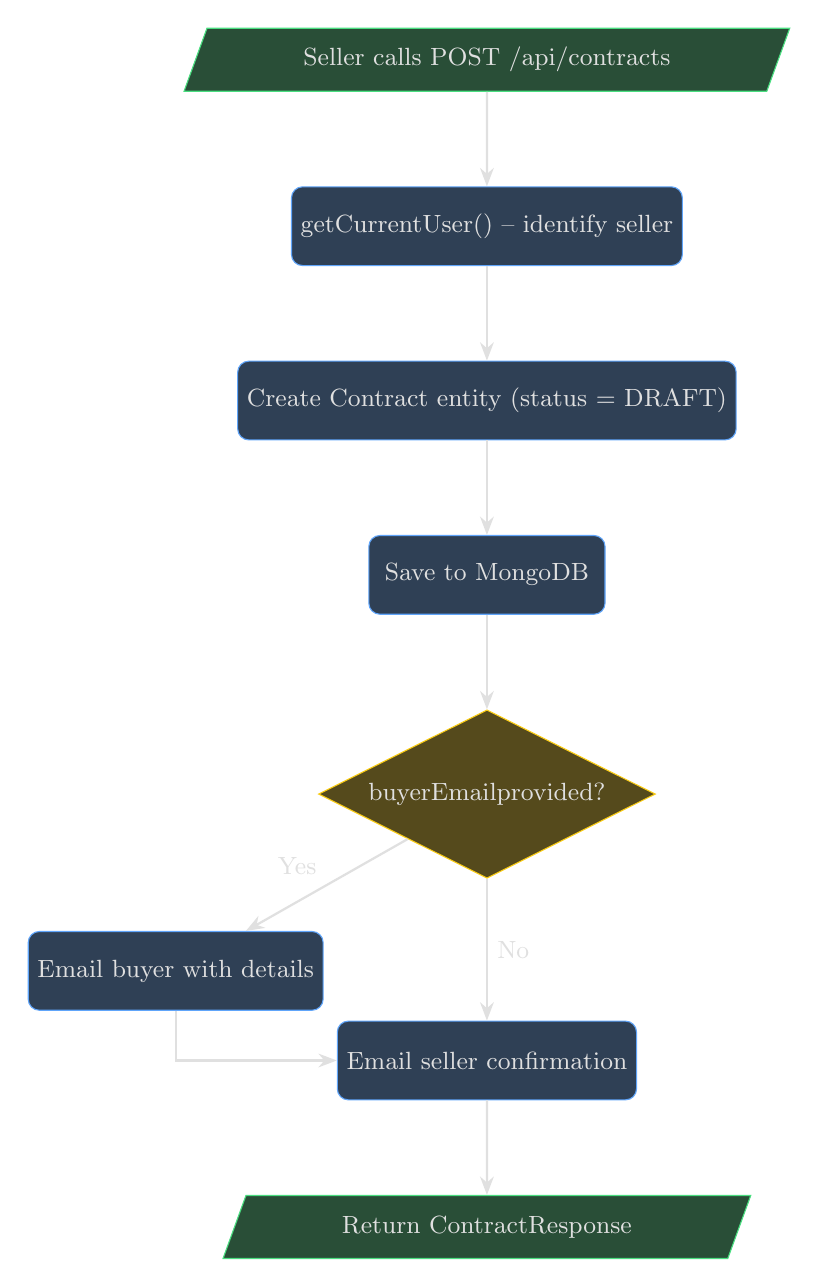
\begin{tikzpicture}[node distance=1.2cm, every node/.style={text=textmain, font=\small}]
    \node[io] (input) {Seller calls POST /api/contracts};
    \node[process, below=of input] (auth) {getCurrentUser() -- identify seller};
    \node[process, below=of auth] (create) {Create Contract entity (status = DRAFT)};
    \node[process, below=of create] (save) {Save to MongoDB};
    \node[decision, below=of save] (buyer) {buyerEmail\\provided?};
    \node[process, below left=1.2cm and 1cm of buyer] (emailbuyer) {Email buyer with details};
    \node[process, below=1.8cm of buyer] (emailseller) {Email seller confirmation};
    \node[io, below=of emailseller] (resp) {Return ContractResponse};
    
    \draw[arrow] (input) -- (auth);
    \draw[arrow] (auth) -- (create);
    \draw[arrow] (create) -- (save);
    \draw[arrow] (save) -- (buyer);
    \draw[arrow] (buyer) -- node[above left] {Yes} (emailbuyer);
    \draw[arrow] (emailbuyer) |- (emailseller);
    \draw[arrow] (buyer) -- node[right] {No} (emailseller);
    \draw[arrow] (emailseller) -- (resp);
\end{tikzpicture}
\caption{Create Contract Flow}
\end{figure}

\subsubsection{acceptContract() -- Buyer Accepts \& Pays}

\begin{figure}[H]
\centering
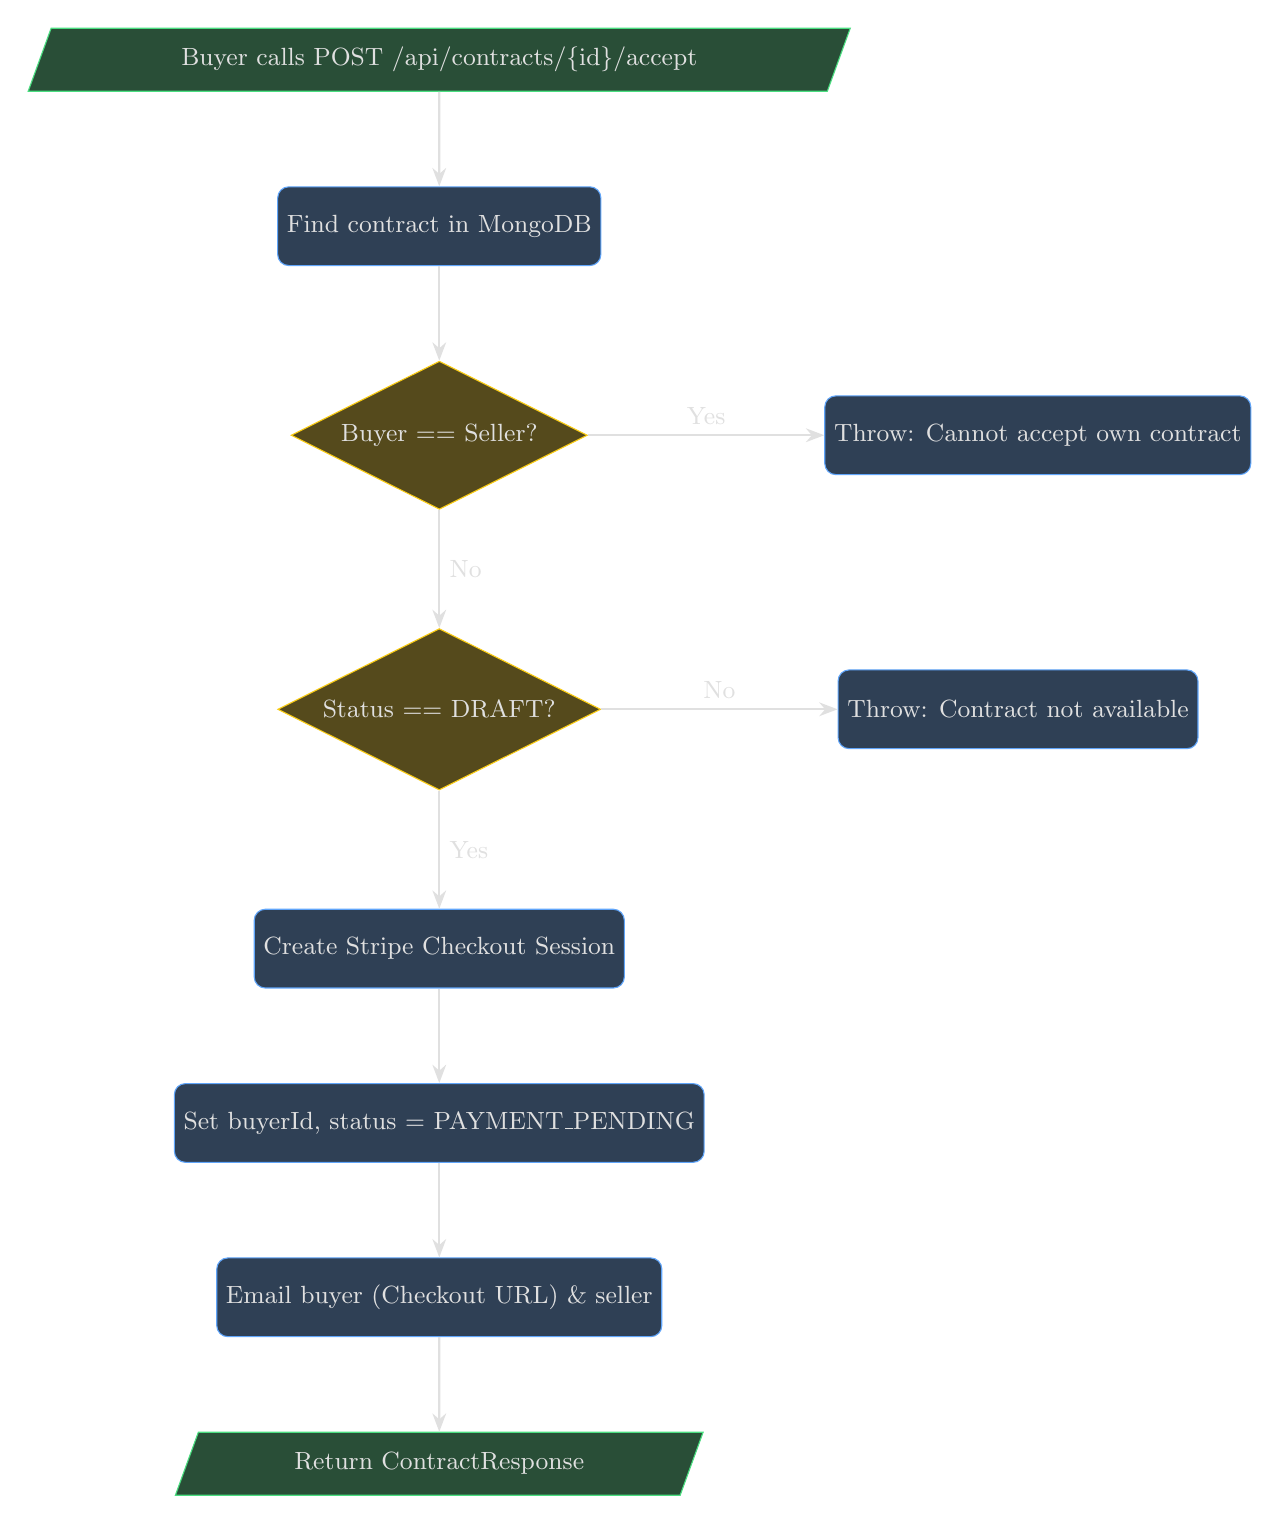
\begin{tikzpicture}[node distance=1.2cm, every node/.style={text=textmain, font=\small}]
    \node[io] (input) {Buyer calls POST /api/contracts/\{id\}/accept};
    \node[process, below=of input] (find) {Find contract in MongoDB};
    \node[decision, below=of find] (own) {Buyer == Seller?};
    \node[process, right=3cm of own] (reject) {Throw: Cannot accept own contract};
    \node[decision, below=1.5cm of own] (status) {Status == DRAFT?};
    \node[process, right=3cm of status] (reject2) {Throw: Contract not available};
    \node[process, below=1.5cm of status] (stripe) {Create Stripe Checkout Session};
    \node[process, below=of stripe] (update) {Set buyerId, status = PAYMENT\_PENDING};
    \node[process, below=of update] (email) {Email buyer (Checkout URL) \& seller};
    \node[io, below=of email] (resp) {Return ContractResponse};
    
    \draw[arrow] (input) -- (find);
    \draw[arrow] (find) -- (own);
    \draw[arrow] (own) -- node[above] {Yes} (reject);
    \draw[arrow] (own) -- node[right] {No} (status);
    \draw[arrow] (status) -- node[above] {No} (reject2);
    \draw[arrow] (status) -- node[right] {Yes} (stripe);
    \draw[arrow] (stripe) -- (update);
    \draw[arrow] (update) -- (email);
    \draw[arrow] (email) -- (resp);
\end{tikzpicture}
\caption{Accept Contract Flow}
\end{figure}

\subsection{PaymentService (Stripe Integration)}

\begin{lstlisting}[caption={PaymentService.java -- Creating a Stripe Checkout Session}]
@Service
public class PaymentService {

    @Value("${stripe.key.secret}")
    private String secretKey;

    @PostConstruct
    public void init() {
        Stripe.apiKey = secretKey;  // Set API key once at startup
    }

    public Session createCheckoutSession(Double amount, String contractId,
                                          String buyerId, String title)
            throws StripeException {
        long amountInPaise = (long) (amount * 100); // Stripe uses smallest unit

        SessionCreateParams params = SessionCreateParams.builder()
            .setMode(SessionCreateParams.Mode.PAYMENT)
            .setSuccessUrl(appBaseUrl + "/swagger-ui/index.html")
            .setCancelUrl(appBaseUrl + "/swagger-ui/index.html")
            .addLineItem(
                SessionCreateParams.LineItem.builder()
                    .setQuantity(1L)
                    .setPriceData(
                        SessionCreateParams.LineItem.PriceData.builder()
                            .setCurrency("inr")
                            .setUnitAmount(amountInPaise)
                            .setProductData(/* title */)
                            .build())
                    .build())
            .setPaymentIntentData(
                SessionCreateParams.PaymentIntentData.builder()
                    .putMetadata("contractId", contractId) // KEY!
                    .build())
            .build();

        return Session.create(params);
    }
}
\end{lstlisting}

\begin{warningbox}{Why \texttt{putMetadata("contractId", contractId)}?}
This is crucial! When Stripe sends the webhook later, we need to know \textit{which contract} the payment was for. By attaching the contractId as metadata to the PaymentIntent, Stripe includes it in the webhook payload, and we can look up the exact contract to update.
\end{warningbox}

\subsection{EmailService (Gmail SMTP Integration)}

\begin{lstlisting}[caption={EmailService.java -- Asynchronous Email Sending}]
@Service
@RequiredArgsConstructor
public class EmailService {

    private final JavaMailSender mailSender;

    @Value("${spring.mail.username:}")
    private String fromEmail;

    @Async  // Runs in a separate thread (non-blocking)
    public void sendEmail(String toEmail, String subject, String body) {
        if (toEmail == null) {
            log.warn("Cannot send mail. Recipient is null");
            return;
        }

        SimpleMailMessage message = new SimpleMailMessage();
        message.setFrom(fromEmail);
        message.setTo(toEmail);
        message.setSubject(subject);
        message.setText(body);

        mailSender.send(message);  // Sends via Gmail SMTP
    }
}
\end{lstlisting}

\begin{interviewbox}{Why is sendEmail() annotated with @Async?}
Sending an email via SMTP can take 2--5 seconds (network handshake, DNS lookup, SMTP authentication). Without \texttt{@Async}, the API response would be \textbf{blocked} for those 2--5 seconds while the email sends.

With \texttt{@Async}, Spring runs \texttt{sendEmail()} in a \textbf{separate background thread}. The API response returns instantly to the user, and the email sends in the background. This is enabled by the \texttt{@EnableAsync} annotation on the main application class.
\end{interviewbox}

\subsection{CustomUserDetailsService}

This service bridges your \texttt{User} entity with Spring Security's internal \texttt{UserDetails} interface.

\begin{lstlisting}[caption={CustomUserDetailsService.java}]
@Service
@RequiredArgsConstructor
public class CustomUserDetailsService implements UserDetailsService {

    private final UserRepository userRepository;

    @Override
    public UserDetails loadUserByUsername(String email)
            throws UsernameNotFoundException {
        // 1. Find the user in MongoDB
        User user = userRepository.findByEmail(email)
                .orElseThrow(() -> new UsernameNotFoundException("Not found"));

        // 2. Convert to Spring Security's User object
        return new org.springframework.security.core.userdetails.User(
                user.getEmail(),
                user.getPassword(),
                new ArrayList<>()  // Authorities/Roles (simplified)
        );
    }
}
\end{lstlisting}


% ============================================================
% CHAPTER 6: ERROR HANDLING
% ============================================================
\section{Error Handling}

Instead of letting raw Java stack traces leak to the API consumer, a \texttt{GlobalExceptionHandler} catches all exceptions and converts them into clean, structured JSON responses.

\begin{lstlisting}[caption={GlobalExceptionHandler.java -- Centralized Error Handling}]
@RestControllerAdvice
public class GlobalExceptionHandler {

    // 404 Not Found
    @ExceptionHandler(ResourceNotFoundException.class)
    public ResponseEntity<ErrorResponse> handleNotFound(
            ResourceNotFoundException ex) {
        ErrorResponse error = ErrorResponse.builder()
            .status(404).error("Not Found")
            .message(ex.getMessage())
            .timestamp(LocalDateTime.now()).build();
        return new ResponseEntity<>(error, HttpStatus.NOT_FOUND);
    }

    // 400 Bad Request (business rule violations)
    @ExceptionHandler(IllegalStateException.class)
    public ResponseEntity<ErrorResponse> handleBadRequest(
            IllegalStateException ex) { /* ... */ }

    // 400 Validation Errors (e.g., @NotBlank failed)
    @ExceptionHandler(MethodArgumentNotValidException.class)
    public ResponseEntity<ErrorResponse> handleValidation(
            MethodArgumentNotValidException ex) { /* ... */ }

    // 409 Conflict (Optimistic Locking)
    @ExceptionHandler(OptimisticLockingFailureException.class)
    public ResponseEntity<ErrorResponse> handleConflict(
            OptimisticLockingFailureException ex) { /* ... */ }

    // 500 Internal Server Error (catch-all)
    @ExceptionHandler(Exception.class)
    public ResponseEntity<ErrorResponse> handleGeneric(Exception ex) {
        // Logs the full stack trace but returns a generic message
        // to avoid leaking internal details to the API consumer.
    }
}
\end{lstlisting}

\begin{examplebox}{Error Response JSON}
When a user tries to accept a contract that is already locked:
\begin{lstlisting}[style=yamlstyle]
{
    "status": 400,
    "error": "Bad Request",
    "message": "This contract is not available. current status: LOCKED",
    "timestamp": "2026-06-20T18:30:45"
}
\end{lstlisting}
\end{examplebox}

\begin{conceptbox}{Optimistic Locking (Version Field)}
The \texttt{Contract} entity has a \texttt{@Version} field. When two users try to modify the same contract simultaneously, MongoDB detects the conflict (the version number doesn't match), and Spring throws an \texttt{OptimisticLockingFailureException}. The handler returns a 409 Conflict, telling the client to retry.

This prevents race conditions like: Buyer clicks ``Satisfy'' and Seller clicks ``Ship'' at the exact same time.
\end{conceptbox}


% ============================================================
% CHAPTER 7: REPOSITORIES
% ============================================================
\section{Repositories (Data Access Layer)}

Repositories are interfaces that Spring Data MongoDB auto-implements at runtime. You just define the method signature, and Spring generates the query.

\begin{lstlisting}[caption={UserRepository.java}]
public interface UserRepository extends MongoRepository<User, String> {
    Optional<User> findByEmail(String email);
    boolean existsByEmail(String email);
}
\end{lstlisting}

\begin{lstlisting}[caption={ContractRepository.java}]
@Repository
public interface ContractRepository
        extends MongoRepository<Contract, String> {
    // Find all contracts where user is seller
    List<Contract> findBySellerId(String sellerId);

    // Find all contracts where user is either seller OR buyer
    List<Contract> findBySellerIdOrBuyerId(String sellerId, String buyerId);

    // Find delivered contracts older than 14 days (for auto-release)
    List<Contract> findByStatusAndTrackingDetailsDeliveryDateBefore(
        ContractStatus status, LocalDateTime cutoffDate);
}
\end{lstlisting}

\begin{interviewbox}{How does \texttt{findByStatusAndTrackingDetailsDeliveryDateBefore} work?}
Spring Data parses the method name and generates a MongoDB query:
\begin{lstlisting}[style=yamlstyle]
{ "status": "DELIVERED",
  "trackingDetails.deliveryDate": { "$lt": cutoffDate } }
\end{lstlisting}
It traverses the embedded document (\texttt{trackingDetails}) using the dot notation. No manual query writing needed!
\end{interviewbox}


% ============================================================
% CHAPTER 8: SCHEDULER
% ============================================================
\section{Background Scheduler (Auto-Release)}

The scheduler runs a background cron job every day at midnight to automatically release funds for contracts that have been delivered for more than 14 days without any dispute.

\begin{lstlisting}[caption={ContractScheduler.java}]
@Component
@RequiredArgsConstructor
public class ContractScheduler {

    public final ContractRepository contractRepository;
    public final ContractService contractService;

    @Scheduled(cron = "0 0 0 * * ?")  // Every day at midnight
    public void processAutoRelease() {
        log.info("Running Auto-Release Scheduler...");

        // Calculate the cutoff: 14 days ago
        LocalDateTime cutoffDate = LocalDateTime.now().minusDays(14);

        // Find all DELIVERED contracts with delivery date > 14 days ago
        List<Contract> expiredContracts = contractRepository
            .findByStatusAndTrackingDetailsDeliveryDateBefore(
                ContractStatus.DELIVERED, cutoffDate);

        for (Contract contract : expiredContracts) {
            // Mark as AUTO_RELEASED (same as satisfied, but automatic)
            contractService.markAsSatisfiedInternal(
                contract, ContractStatus.AUTO_RELEASED);
        }
    }
}
\end{lstlisting}

\begin{conceptbox}{Cron Expression: \texttt{0 0 0 * * ?}}
\begin{center}
\begin{tabular}{cccccc}
\texttt{0} & \texttt{0} & \texttt{0} & \texttt{*} & \texttt{*} & \texttt{?} \\
\small{second} & \small{minute} & \small{hour} & \small{day} & \small{month} & \small{day-of-week} \\
\end{tabular}
\end{center}
This means: At second 0, minute 0, hour 0 (midnight), every day, every month, any day of the week. Enabled by \texttt{@EnableScheduling} on the main application class.
\end{conceptbox}


% ============================================================
% CHAPTER 9: DTOs
% ============================================================
\section{Data Transfer Objects (DTOs)}

DTOs define the shape of data that enters and leaves the API. They act as a contract between the frontend and backend.

\subsection{Why Use DTOs Instead of Entities Directly?}

\begin{warningbox}{Security Risk Without DTOs}
If you return the \texttt{User} entity directly from the login endpoint, the JSON response would include the \textbf{hashed password}! DTOs let you control exactly which fields are exposed to the client.
\end{warningbox}

\subsection{Request DTOs (Incoming Data)}

\begin{longtable}{@{}lp{8cm}@{}}
\toprule
\textbf{DTO} & \textbf{Fields \& Validations} \\
\midrule
\texttt{RegisterRequest} & \texttt{name} (@NotBlank), \texttt{email} (@NotBlank, @Email), \texttt{password} (@NotBlank, @Size min=6) \\
\texttt{LoginRequest} & \texttt{email} (@NotBlank), \texttt{password} (@NotBlank) \\
\texttt{CreateContractRequest} & \texttt{title} (@NotBlank), \texttt{description} (@NotBlank), \texttt{amount} (@Min 1), \texttt{buyerEmail} (@Email, optional) \\
\texttt{ShipContractRequest} & \texttt{trackingId} (@NotBlank), \texttt{logisticsProvider} (@NotBlank) \\
\texttt{RaiseDisputeRequest} & \texttt{reason} (@NotBlank) \\
\bottomrule
\end{longtable}

\subsection{Response DTOs (Outgoing Data)}

\begin{longtable}{@{}lp{8cm}@{}}
\toprule
\textbf{DTO} & \textbf{Fields} \\
\midrule
\texttt{AuthResponse} & \texttt{token} (JWT string) \\
\texttt{UserResponse} & \texttt{id}, \texttt{name}, \texttt{email}, \texttt{role}, \texttt{createdAt} \\
\texttt{ContractResponse} & \texttt{id}, \texttt{sellerId}, \texttt{buyerId}, \texttt{title}, \texttt{description}, \texttt{amount}, \texttt{status}, \texttt{trackingDetails}, \texttt{paymentIntentId}, \texttt{createdAt}, \texttt{updatedAt}, \texttt{version} \\
\texttt{ErrorResponse} & \texttt{status}, \texttt{error}, \texttt{message}, \texttt{timestamp} \\
\bottomrule
\end{longtable}


% ============================================================
% CHAPTER 10: EXTERNAL INTEGRATIONS
% ============================================================
\section{External Integrations}

\subsection{Integration Architecture}

\begin{figure}[H]
\centering
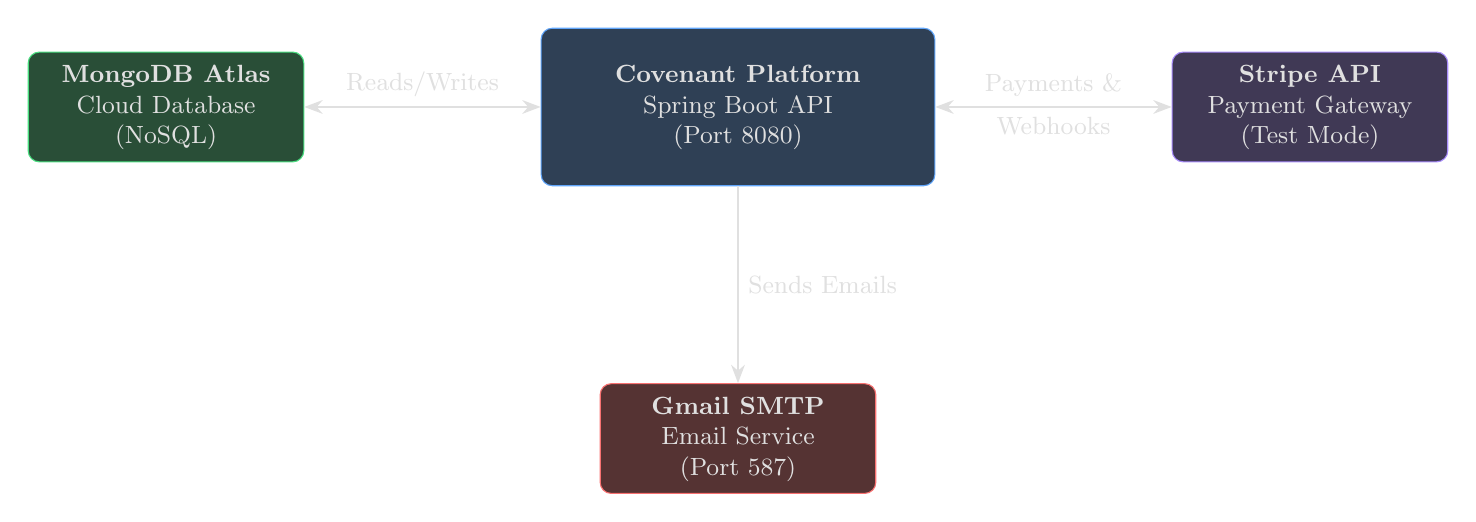
\begin{tikzpicture}[node distance=2cm, every node/.style={text=textmain, font=\small}]
    % Center
    \node[process, minimum width=5cm, minimum height=2cm, fill=covenantblue!25!pagebg] (api) {
        \begin{tabular}{c}
            \textbf{Covenant Platform} \\
            Spring Boot API \\
            (Port 8080)
        \end{tabular}
    };
    
    % MongoDB
    \node[process, left=3cm of api, fill=successgreen!25!pagebg, draw=successgreen, minimum width=3.5cm] (mongo) {
        \begin{tabular}{c}
            \textbf{MongoDB Atlas} \\
            Cloud Database \\
            (NoSQL)
        \end{tabular}
    };
    
    % Stripe
    \node[process, right=3cm of api, fill=keywordcolor!25!pagebg, draw=keywordcolor, minimum width=3.5cm] (stripe) {
        \begin{tabular}{c}
            \textbf{Stripe API} \\
            Payment Gateway \\
            (Test Mode)
        \end{tabular}
    };
    
    % Gmail
    \node[process, below=2.5cm of api, fill=dangerred!25!pagebg, draw=dangerred, minimum width=3.5cm] (gmail) {
        \begin{tabular}{c}
            \textbf{Gmail SMTP} \\
            Email Service \\
            (Port 587)
        \end{tabular}
    };
    
    % Arrows
    \draw[arrow, <->] (api) -- node[above] {Reads/Writes} (mongo);
    \draw[arrow, <->] (api) -- node[above] {Payments \&} node[below] {Webhooks} (stripe);
    \draw[arrow, ->] (api) -- node[right] {Sends Emails} (gmail);
\end{tikzpicture}
\caption{External Integration Architecture}
\end{figure}

\subsection{MongoDB Atlas}

\begin{itemize}
    \item \textbf{Connection}: Via \texttt{MONGODB\_URI} environment variable (connection string with credentials).
    \item \textbf{Driver}: Spring Data MongoDB auto-configures the connection pool.
    \item \textbf{Database name}: \texttt{covenant} (configured in \texttt{application.yaml}).
    \item \textbf{Collections}: \texttt{users} and \texttt{contract} (auto-created on first write).
\end{itemize}

\subsection{Stripe Payment Gateway}

\subsubsection{Payment Flow (End-to-End)}

\begin{figure}[H]
\centering
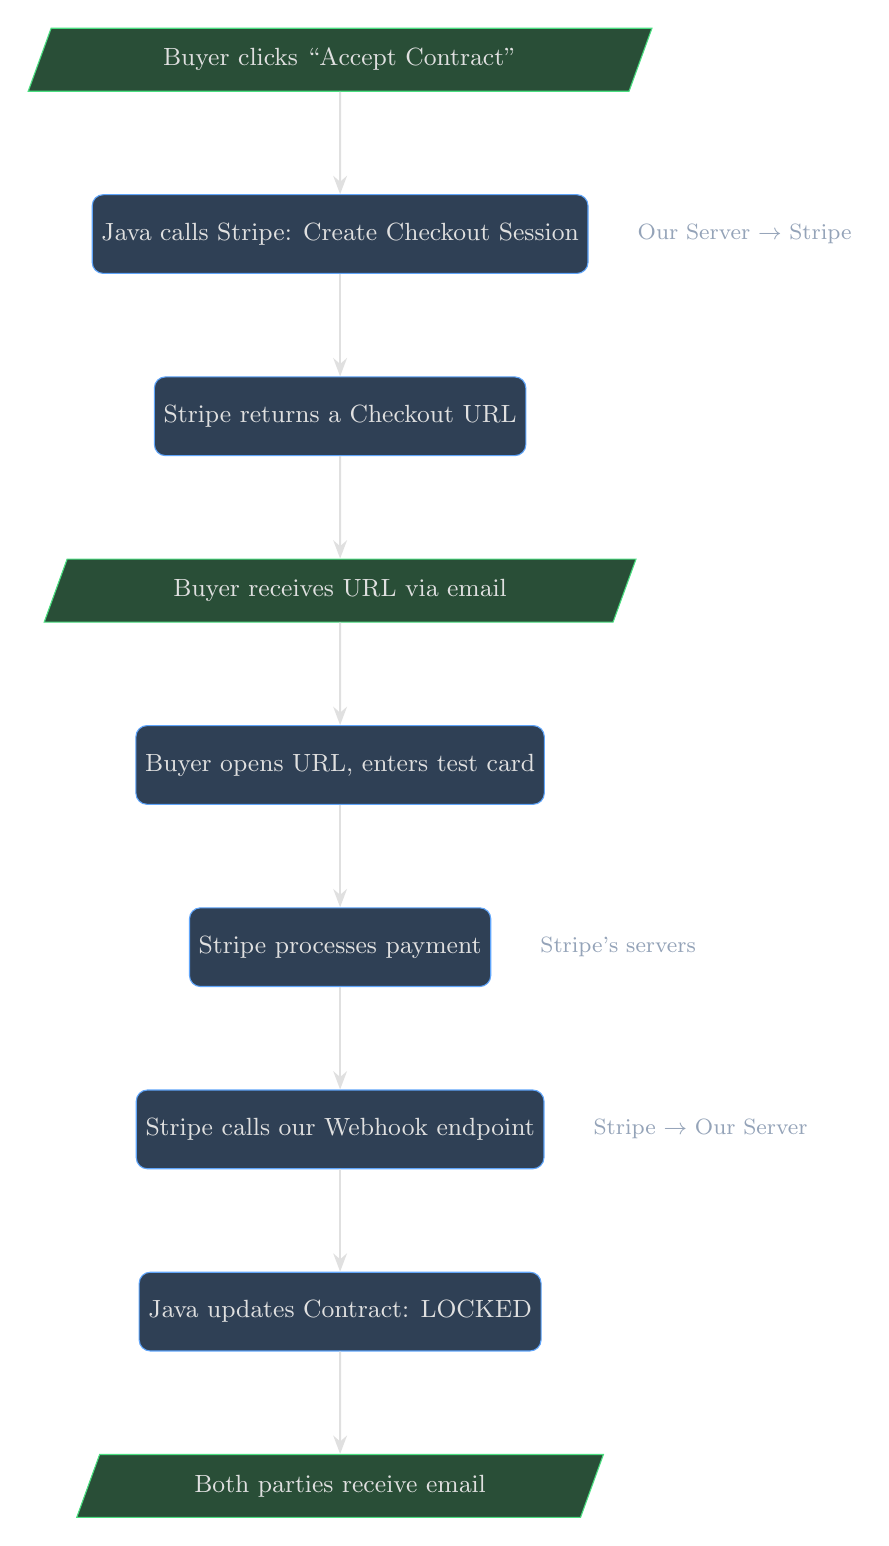
\begin{tikzpicture}[node distance=1.3cm, every node/.style={text=textmain, font=\footnotesize}]
    \node[io] (start) {Buyer clicks ``Accept Contract''};
    \node[process, below=of start] (create) {Java calls Stripe: Create Checkout Session};
    \node[process, below=of create] (url) {Stripe returns a Checkout URL};
    \node[io, below=of url] (email) {Buyer receives URL via email};
    \node[process, below=of email] (pay) {Buyer opens URL, enters test card};
    \node[process, below=of pay] (stripe) {Stripe processes payment};
    \node[process, below=of stripe] (webhook) {Stripe calls our Webhook endpoint};
    \node[process, below=of webhook] (lock) {Java updates Contract: LOCKED};
    \node[io, below=of lock] (notify) {Both parties receive email};
    
    \draw[arrow] (start) -- (create);
    \draw[arrow] (create) -- (url);
    \draw[arrow] (url) -- (email);
    \draw[arrow] (email) -- (pay);
    \draw[arrow] (pay) -- (stripe);
    \draw[arrow] (stripe) -- (webhook);
    \draw[arrow] (webhook) -- (lock);
    \draw[arrow] (lock) -- (notify);
    
    % Labels
    \node[right=0.5cm of create, text=covenantgray] {Our Server $\rightarrow$ Stripe};
    \node[right=0.5cm of stripe, text=covenantgray] {Stripe's servers};
    \node[right=0.5cm of webhook, text=covenantgray] {Stripe $\rightarrow$ Our Server};
\end{tikzpicture}
\caption{Complete Stripe Payment Flow}
\end{figure}

\subsubsection{Why Webhooks are Essential}

\begin{conceptbox}{The Browser Redirect Problem}
After paying, Stripe redirects the buyer's browser to our ``success'' URL. But what if:
\begin{itemize}
    \item The buyer's internet drops during the redirect?
    \item The buyer closes the browser tab before the redirect?
    \item A malicious user manually types in the success URL without paying?
\end{itemize}
In all these cases, our server would never know the payment succeeded. That's why Stripe makes a \textbf{direct server-to-server call} (webhook) to guarantee delivery of the payment confirmation.
\end{conceptbox}

\subsubsection{Webhook Security: Signature Verification}

When Stripe calls our webhook, it includes a \texttt{Stripe-Signature} header. Our server uses the \texttt{STRIPE\_WEBHOOK\_SECRET} to verify this signature, ensuring the request actually came from Stripe and wasn't forged by an attacker.

\subsection{Gmail SMTP}

\begin{longtable}{@{}lp{8cm}@{}}
\toprule
\textbf{Configuration} & \textbf{Value} \\
\midrule
Host & \texttt{smtp.gmail.com} \\
Port & 587 (STARTTLS) \\
Authentication & Gmail App Password (not regular password) \\
TLS Encryption & Enabled (mandatory for Gmail) \\
\bottomrule
\end{longtable}

Emails are sent at 6 points in the contract lifecycle:
\begin{enumerate}
    \item Contract Created (to Seller)
    \item Contract Proposed (to Buyer, if email provided)
    \item Contract Accepted (to Seller + Buyer with Checkout URL)
    \item Payment Confirmed (to Seller)
    \item Item Shipped (to Buyer with tracking ID)
    \item Item Delivered (to Buyer)
    \item Funds Released / Dispute Raised / Dispute Resolved
\end{enumerate}


% ============================================================
% CHAPTER 11: APPLICATION CONFIGURATION
% ============================================================
\section{Application Configuration}

All configuration is externalized via environment variables, following the \textbf{12-Factor App} methodology.

\begin{lstlisting}[style=yamlstyle, caption={application.yaml}]
spring:
  data:
    mongodb:
      uri: ${MONGODB_URI}           # Connection string (from env)
      database: covenant
  mail:
    host: ${EMAIL_HOST:smtp.gmail.com}
    port: ${EMAIL_PORT:587}
    username: ${EMAIL_USERNAME:}     # Gmail address
    password: ${EMAIL_PASSWORD:}     # Gmail App Password

app:
  base-url: ${APP_BASE_URL:http://localhost:8080}

jwt:
  secret: ${JWT_SECRET}             # Base64-encoded HMAC key

stripe:
  key:
    secret: ${STRIPE_SECRET_KEY}
    publishable: ${STRIPE_PUBLISHABLE_KEY}
  webhook:
    secret: ${STRIPE_WEBHOOK_SECRET:}

management:
  endpoints:
    web:
      exposure:
        include: health, info       # Spring Actuator endpoints
\end{lstlisting}

\begin{interviewbox}{What does \texttt{\$\{EMAIL\_HOST:smtp.gmail.com\}} mean?}
The syntax \texttt{\$\{VARIABLE:default\}} means: ``Use the environment variable \texttt{EMAIL\_HOST} if it exists; otherwise, fall back to \texttt{smtp.gmail.com}.'' The colon separates the variable name from the default value. If there's no colon (like \texttt{\$\{JWT\_SECRET\}}), the app will \textbf{fail to start} if the variable is missing.
\end{interviewbox}


% ============================================================
% CHAPTER 12: COMPLETE ESCROW FLOW
% ============================================================
\section{The Complete Escrow Flow}

This chapter ties everything together with a complete end-to-end walkthrough.

\begin{examplebox}{Scenario: Alice sells a laptop to Bob for INR 50,000}
\begin{enumerate}[leftmargin=*]
    \item \textbf{Alice registers}: \texttt{POST /api/auth/register}
        \begin{itemize}
            \item BCrypt hashes her password
            \item User document saved to MongoDB
        \end{itemize}
    
    \item \textbf{Alice logs in}: \texttt{POST /api/auth/login}
        \begin{itemize}
            \item Password verified against hash
            \item JWT token generated (valid 24 hours)
        \end{itemize}
    
    \item \textbf{Alice creates a contract}: \texttt{POST /api/contracts}
        \begin{itemize}
            \item JWT decoded $\rightarrow$ Alice identified as seller
            \item Contract saved with status \texttt{DRAFT}
            \item Bob receives email: ``Contract Proposed: MacBook Pro''
        \end{itemize}
    
    \item \textbf{Bob registers, logs in, and accepts}: \texttt{POST /api/contracts/\{id\}/accept}
        \begin{itemize}
            \item Validation: Bob $\neq$ Alice (can't accept own contract)
            \item Validation: Status must be \texttt{DRAFT}
            \item \texttt{PaymentService} calls Stripe API $\rightarrow$ Checkout Session created
            \item Contract updated: \texttt{buyerId = Bob}, status = \texttt{PAYMENT\_PENDING}
            \item Bob gets email with Stripe Checkout URL
        \end{itemize}
    
    \item \textbf{Bob pays via Stripe}:
        \begin{itemize}
            \item Bob clicks the Checkout URL, enters test card \texttt{4242 4242 4242 4242}
            \item Stripe processes the payment
            \item Stripe calls \texttt{POST /api/webhooks/stripe} (webhook)
            \item \texttt{StripeWebhookController} verifies the signature
            \item Extracts \texttt{contractId} from metadata
            \item Calls \texttt{confirmPaymentInternal()} $\rightarrow$ status = \texttt{LOCKED}
            \item Alice gets email: ``Payment Received! Please ship.''
        \end{itemize}
    
    \item \textbf{Alice ships the laptop}: \texttt{PATCH /api/contracts/\{id\}/ship}
        \begin{itemize}
            \item Tracking details saved (ID + provider)
            \item Status changes to \texttt{SHIPPED}
            \item Bob gets email with tracking ID
        \end{itemize}
    
    \item \textbf{Alice marks as delivered}: \texttt{PATCH /api/contracts/\{id\}/delivery}
        \begin{itemize}
            \item Delivery date recorded (starts the 14-day timer)
            \item Status changes to \texttt{DELIVERED}
            \item Bob gets email: ``Please inspect within 14 days''
        \end{itemize}
    
    \item \textbf{Bob is happy}: \texttt{POST /api/contracts/\{id\}/satisfy}
        \begin{itemize}
            \item Status changes to \texttt{SATISFIED}
            \item Alice gets email: ``Funds of INR 50,000 released!''
        \end{itemize}
    
    \item \textbf{Alternative -- Bob does nothing for 14 days}:
        \begin{itemize}
            \item \texttt{ContractScheduler} runs at midnight
            \item Finds contracts with \texttt{deliveryDate} $>$ 14 days ago
            \item Auto-releases funds (status = \texttt{AUTO\_RELEASED})
        \end{itemize}
    
    \item \textbf{Alternative -- Bob is unhappy}: \texttt{POST /api/contracts/\{id\}/dispute}
        \begin{itemize}
            \item Status changes to \texttt{DISPUTED} (funds frozen)
            \item Admin resolves: either \texttt{REFUNDED} or \texttt{SATISFIED}
        \end{itemize}
\end{enumerate}
\end{examplebox}

\subsection{Complete Architecture Diagram}

\begin{figure}[H]
\centering
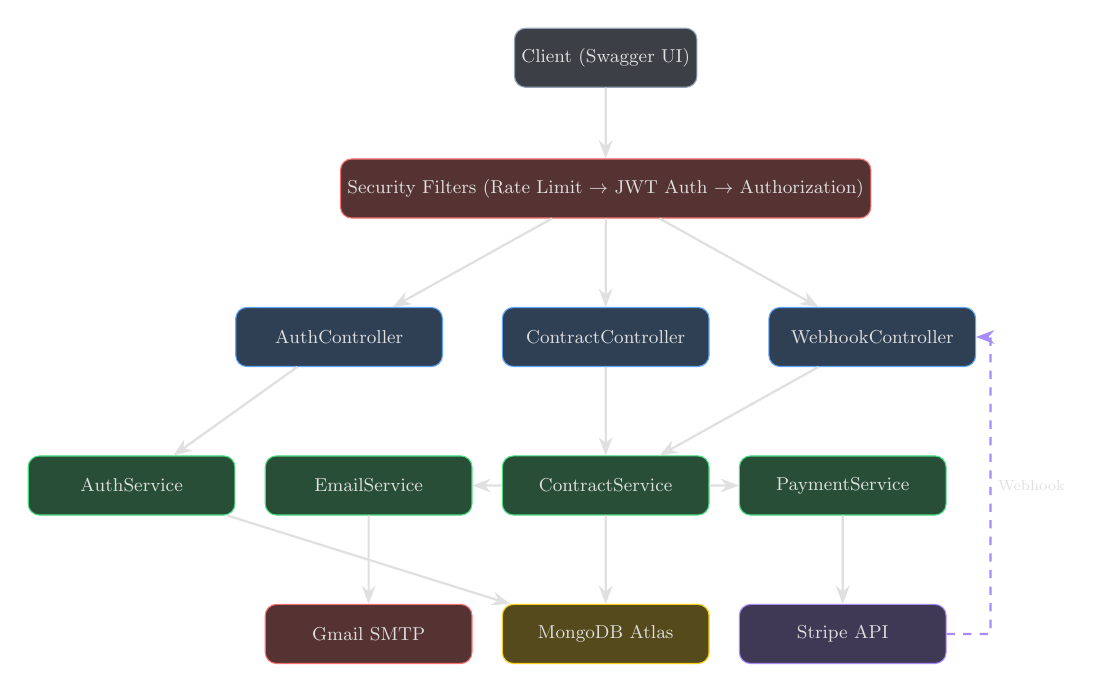
\begin{tikzpicture}[node distance=1.2cm, every node/.style={text=textmain, font=\scriptsize}, scale=0.75, transform shape]
    % Client
    \node[process, minimum width=3cm, fill=covenantgray!25!pagebg, draw=covenantgray] (client) {Client (Swagger UI)};
    
    % Filters
    \node[process, below=of client, minimum width=8cm, fill=dangerred!25!pagebg, draw=dangerred] (filters) {Security Filters (Rate Limit $\rightarrow$ JWT Auth $\rightarrow$ Authorization)};
    
    % Controllers Row
    \node[process, below=1.5cm of filters, minimum width=3.5cm] (contract) {ContractController};
    \node[process, left=1cm of contract, minimum width=3.5cm] (auth) {AuthController};
    \node[process, right=1cm of contract, minimum width=3.5cm] (webhook) {WebhookController};
    
    % Services Row
    \node[process, below=1.5cm of contract, minimum width=3.5cm, fill=successgreen!25!pagebg, draw=successgreen] (contractsvc) {ContractService};
    \node[process, left=0.5cm of contractsvc, minimum width=3.5cm, fill=successgreen!25!pagebg, draw=successgreen] (emailsvc) {EmailService};
    \node[process, left=0.5cm of emailsvc, minimum width=3.5cm, fill=successgreen!25!pagebg, draw=successgreen] (authsvc) {AuthService};
    \node[process, right=0.5cm of contractsvc, minimum width=3.5cm, fill=successgreen!25!pagebg, draw=successgreen] (paysvc) {PaymentService};
    
    % External Row
    \node[process, below=1.5cm of contractsvc, minimum width=3.5cm, fill=warningyellow!25!pagebg, draw=warningyellow] (mongo) {MongoDB Atlas};
    \node[process, below=1.5cm of emailsvc, minimum width=3.5cm, fill=dangerred!25!pagebg, draw=dangerred] (gmail) {Gmail SMTP};
    \node[process, below=1.5cm of paysvc, minimum width=3.5cm, fill=keywordcolor!25!pagebg, draw=keywordcolor] (stripe) {Stripe API};
    
    % Arrows
    \draw[arrow] (client) -- (filters);
    \draw[arrow] (filters) -- (auth);
    \draw[arrow] (filters) -- (contract);
    \draw[arrow] (filters) -- (webhook);
    \draw[arrow] (auth) -- (authsvc);
    \draw[arrow] (contract) -- (contractsvc);
    \draw[arrow] (webhook) -- (contractsvc);
    \draw[arrow] (contractsvc) -- (mongo);
    \draw[arrow] (contractsvc) -- (paysvc);
    \draw[arrow] (contractsvc) -- (emailsvc);
    \draw[arrow] (paysvc) -- (stripe);
    \draw[arrow] (emailsvc) -- (gmail);
    \draw[arrow] (authsvc) -- (mongo);
    
    % Webhook arrow from Stripe back
    \draw[arrow, dashed, keywordcolor] (stripe) -- ++(2.5,0) |- node[near start, right] {Webhook} (webhook);
\end{tikzpicture}
\caption{Complete System Architecture}
\end{figure}


% ============================================================
% CHAPTER 13: KEY DESIGN PATTERNS & CONCEPTS
% ============================================================
\section{Key Design Patterns \& Interview Concepts}

\subsection{Design Patterns Used}

\begin{longtable}{@{}lp{9cm}@{}}
\toprule
\textbf{Pattern} & \textbf{Where It's Used} \\
\midrule
\textbf{Layered Architecture} & Controller $\rightarrow$ Service $\rightarrow$ Repository separation \\
\textbf{DTO Pattern} & Request/Response DTOs isolate API contract from internal entities \\
\textbf{Builder Pattern} & Lombok's \texttt{@Builder} on Response DTOs and TrackingDetails \\
\textbf{Repository Pattern} & Spring Data MongoDB interfaces abstract database access \\
\textbf{Filter Chain Pattern} & Security filters (Rate Limit $\rightarrow$ JWT $\rightarrow$ Authorization) \\
\textbf{Strategy Pattern} & Different status transitions handled by different methods \\
\textbf{State Machine} & ContractStatus enum manages valid state transitions \\
\textbf{Observer/Webhook} & Stripe notifies our server asynchronously on payment events \\
\textbf{Template Method} & \texttt{OncePerRequestFilter} provides the template, we override \texttt{doFilterInternal} \\
\bottomrule
\end{longtable}

\subsection{Key Annotations Explained}

\begin{longtable}{@{}lp{9cm}@{}}
\toprule
\textbf{Annotation} & \textbf{What It Does} \\
\midrule
\texttt{@SpringBootApplication} & Combines \texttt{@Configuration}, \texttt{@EnableAutoConfiguration}, \texttt{@ComponentScan}. The entry point. \\
\texttt{@RestController} & Marks a class as a REST API controller. All methods return JSON. \\
\texttt{@Service} & Marks a class as a business logic component. Spring manages its lifecycle. \\
\texttt{@Repository} & Marks an interface for database access. Spring auto-implements it. \\
\texttt{@Component} & Generic Spring-managed bean (used for filters, schedulers). \\
\texttt{@RequiredArgsConstructor} & Lombok generates a constructor with all \texttt{final} fields. Enables constructor injection. \\
\texttt{@Data} & Lombok generates getters, setters, \texttt{toString()}, \texttt{equals()}, \texttt{hashCode()}. \\
\texttt{@Transactional} & Wraps the method in a database transaction. Rollback on exception. \\
\texttt{@Async} & Runs the method in a separate thread (non-blocking). \\
\texttt{@Scheduled} & Runs the method on a cron schedule (background job). \\
\texttt{@Value} & Injects values from \texttt{application.yaml} or environment variables. \\
\texttt{@PostConstruct} & Runs once after the bean is created and dependencies are injected. \\
\texttt{@Valid} & Triggers Jakarta Bean Validation on the annotated parameter. \\
\bottomrule
\end{longtable}

\subsection{Common Interview Questions}

\begin{interviewbox}{Questions You Should Be Ready For}
\begin{enumerate}
    \item \textbf{JWT}: ``What happens if a JWT is stolen? How would you revoke it?''
    \item \textbf{BCrypt}: ``Why not use SHA-256 or MD5 for password hashing?''
    \item \textbf{MongoDB vs SQL}: ``Why did you choose MongoDB for financial data?''
    \item \textbf{Webhooks}: ``Why not just check the payment status when the user is redirected?''
    \item \textbf{@Async}: ``What happens if the email fails? Does the API return an error?''
    \item \textbf{Rate Limiting}: ``What is the Token Bucket algorithm?''
    \item \textbf{Optimistic Locking}: ``What if two users modify the same contract simultaneously?''
    \item \textbf{@Transactional}: ``What happens if an exception is thrown mid-transaction?''
    \item \textbf{Stateless}: ``Why stateless JWT instead of session-based auth?''
    \item \textbf{CSRF}: ``Why did you disable CSRF protection?''
\end{enumerate}
\end{interviewbox}


% ============================================================
% APPENDIX
% ============================================================
\appendix
\section{Environment Variables Reference}

\begin{longtable}{@{}lp{8cm}@{}}
\toprule
\textbf{Variable} & \textbf{Description} \\
\midrule
\texttt{MONGODB\_URI} & Full MongoDB Atlas connection string \\
\texttt{JWT\_SECRET} & Base64-encoded secret key for signing JWTs \\
\texttt{STRIPE\_SECRET\_KEY} & Stripe test-mode secret key (starts with \texttt{sk\_test\_}) \\
\texttt{STRIPE\_PUBLISHABLE\_KEY} & Stripe test-mode publishable key \\
\texttt{STRIPE\_WEBHOOK\_SECRET} & Webhook signing secret (starts with \texttt{whsec\_}) \\
\texttt{EMAIL\_USERNAME} & Gmail address used to send emails \\
\texttt{EMAIL\_PASSWORD} & Gmail App Password (16-character code) \\
\texttt{APP\_BASE\_URL} & Public URL of the deployed API \\
\bottomrule
\end{longtable}

\section{API Endpoints Quick Reference}

\begin{longtable}{@{}llll@{}}
\toprule
\textbf{Method} & \textbf{Endpoint} & \textbf{Auth} & \textbf{Actor} \\
\midrule
POST & /api/auth/register & Public & Anyone \\
POST & /api/auth/login & Public & Anyone \\
GET & /api/contracts & JWT & Any User \\
POST & /api/contracts & JWT & Seller \\
GET & /api/contracts/\{id\} & JWT & Party/Admin \\
POST & /api/contracts/\{id\}/accept & JWT & Buyer \\
POST & /api/contracts/\{id\}/confirm-payment & JWT & Buyer \\
PATCH & /api/contracts/\{id\}/ship & JWT & Seller \\
PATCH & /api/contracts/\{id\}/delivery & JWT & Seller \\
POST & /api/contracts/\{id\}/satisfy & JWT & Buyer \\
POST & /api/contracts/\{id\}/cancel & JWT & Seller \\
POST & /api/contracts/\{id\}/dispute & JWT & Buyer \\
POST & /api/contracts/\{id\}/resolve?refundBuyer=true & JWT & Admin \\
POST & /api/webhooks/stripe & Public & Stripe \\
\bottomrule
\end{longtable}

\end{document}
